%-  LaTeX source file

%-  section4.tex ~~
%
%   This is the fourth section of the paper.
%
%                                                   ~~ last updated 22 Sep 2019

%%%%%%%%%%%%%%%%%%%%%%%%%%%%%%%%%%%%%%%%%%%%%%%%%%%%%%%%%%%%%%%%%%%%%%%%%%%%%%%

As outlined in Section~\ref{subsec:panda-at-olcf}, the BigPanDA team operated
under several OLCF project identifiers, including CSC108, a DD project which
sought to take advantage of ``backfill mode'' in order to consume unutilized
resources on Titan which would otherwise have gone to waste, without affecting
other projects' quality of service. The focus of this section is to assess the
degree to which CSC108 accomplished that goal and especially to analyze the
impact the project made on Titan.

\jhanote{there is a difference between ``idle'' and ``unutilized''. Need more
rigour in the definition of the stated goals}
\seannote{I admit I don't know the difference. What I generally intend is to
refer to machine which are available to perform work but aren't working.}
\jhanote{Idle is a state when not running. Underutilized is a ``response'' measured against a notion of adequate or desired utilization.}

% \jhanote{slightly misleading to claim there are three queues then to say
% immediately there is no backfill queue. Haven't we already discussed this in
% Section 3?}
% \seannote{It was confusing as written, so I moved the discussion of queues into
% Section 3.2. There was no backfill queue -- backfill was an optional feature
% that could be added to existing queues, and we played fast and loose in the
% past with how we referred to a ``queue'' that didn't actually exist.}

As a convention, we will sometimes make use of a common scheduling metaphor in
which jobs waiting to run on a computer are represented by rocks that are being
used to fill a jar. Capability class jobs on Titan are the largest rocks, and
the scheduler typically fills the remaining space around the largest rocks
with smaller rocks. CSC108 attempted to fill whatever space remains, thanks
to its having been given the lowest possible priority.

%%%%%%%%%%%%%%%%%%%%%%%%%%%%%%%%%%%%%%%%%%%%%%%%%%%%%%%%%%%%%%%%%%%%%%%%%%%%%%%%
\subsection{Rescheduling study}
\label{subsec:rescheduling-study}

% \jhanote{Please make the formulation of the statement more precise}
% \seannote{I'm not sure I made it any better, but I tried.} 

\jhanote{the following is a very strong statement. Discuss}

Recall that the goal of CSC108 was to consume unutilized resources on Titan
that would otherwise have remained unutilized, without decreasing the quality
of service experienced by other projects on Titan.  As shown in
Figure~\ref{fig:monthly-consumption}, CSC108 consumed hundreds of millions of
core hours on Titan. These resources are guaranteed to have been unutilized at
the time of that CSC108's jobs were scheduled because during that time period,
there was no pre-emption in the batch queue on Titan. Moreover, even if Moab
had ended running jobs in order to run other jobs with higher priorities
instead, CSC108's jobs would never have been used to replace existing jobs
because of the custom policies in place that guaranteed CSC108 would always
have the lowest priority on Titan. Therefore, CSC108 consumed millions of core
hours on Titan, all of which were guaranteed to have been unutilized at the
time that CSC108's jobs were scheduled.

It is a more difficult problem, however, to prove that these unutilized
resources on Titan would have remained unutilized and therefore ``gone to
waste''. For example, although the resources were unutilized at the time that
CSC108's jobs were scheduled, if other projects submitted jobs to Titan before
CSC108's jobs completed, then CSC108's jobs could be said to have ``blocked''
other jobs from running. This competition for resources would immediately imply
that, although some of the resources consumed by CSC108 would have gone to
waste, the rest of those resources would not have been wasted.

The simple bar plot shown in Figure~\ref{fig:jacks-slide} seems to show, at
first glance, that utilization by CSC108 has increased at the same time that
utilization by other projects has decreased, which is suggestive of competition
for resources. As a simple way to investigate this competition for resources,
we conducted an experiment in which three years' worth of job traces from Titan
were rescheduled, with and without CSC108's jobs, so that we could estimate
the impact of CSC108's jobs on wait times, throughput, and utilization for
Titan.

\jhanote{Hypothesis as currently formulated needs greater clarity: ``Has no
effect on Titan'' is too casual and clearly wrong, because it does increase
the utilization!} \seannote{I changed it to say ``null hypothesis''. It is
definitely a null hypothesis. The problem then, I suppose, is the implication
then that I will be seeking a p-value to test it.}

% \jhanote{Difficult to read /understand algorithm as is presented.}
% \seannote{I have updated to explain with more words and simpler pseudocode.}
% For two-column wide figures use
\begin{figure*}
% Use the relevant command to insert your figure file.
% For example, with the graphicx package use
  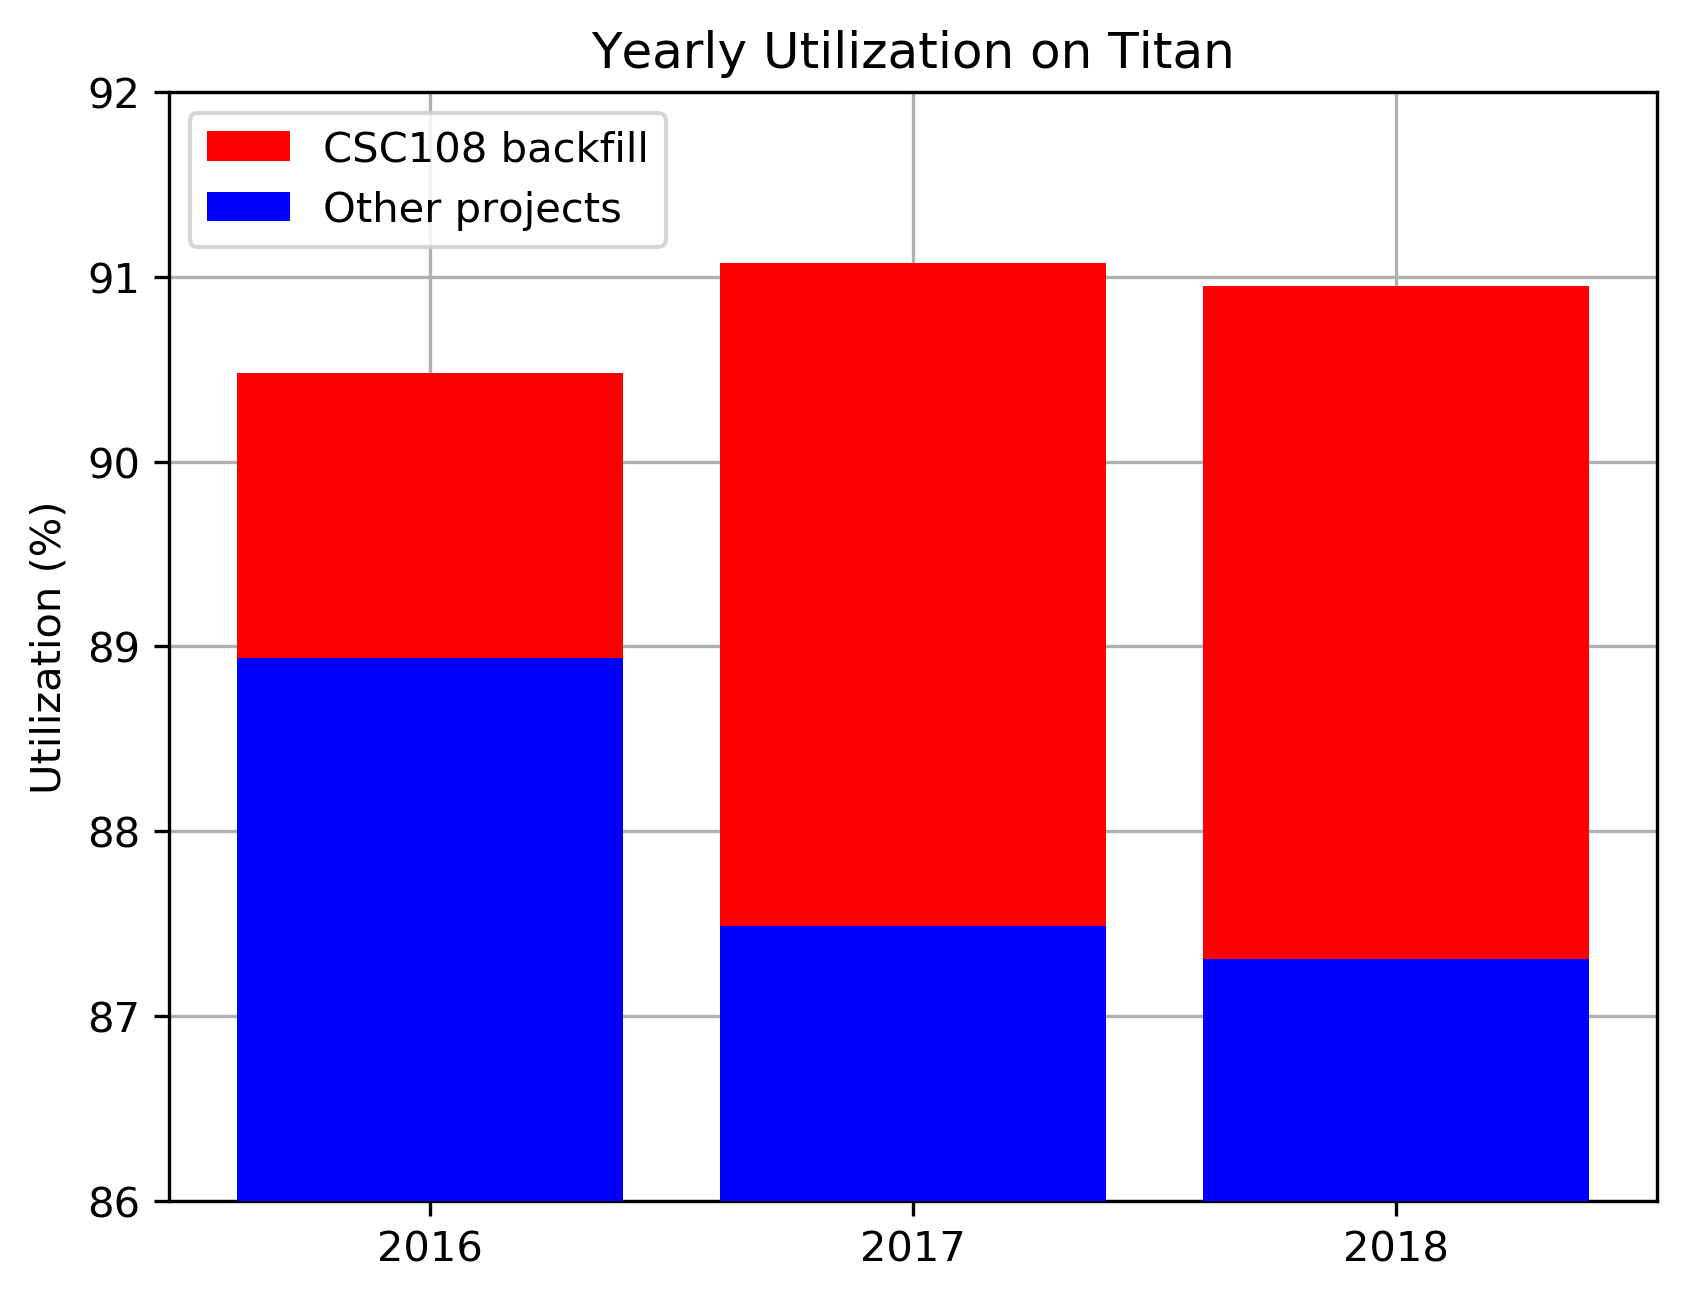
\includegraphics[width=0.75\textwidth]{images/barplot-jacks-slide.png}
% figure caption is below the figure
\caption{This bar plot visualizes the yearly utilization of Titan core hours,
separated into two categories: CSC108's utilization of Titan core hours through
backfill opportunities (shown in red), and all other utilization of core hours
on Titan (shown in blue).}
\label{fig:jacks-slide}
\end{figure*}

What we mean by ``compressing'' job traces is rescheduling the jobs that ran
on Titan while preserving the original execution order, under the assumption of
100\% node availability (all nodes up and running all the time). 

In order to reschedule the jobs, we made a simplifying assumption of 100\% node
availability, meaning that we assumed all of Titan's nodes were up and running
all the time. Original job execution order was also preserved. We rescheduled
the jobs once with CSC108's jobs included and then once with CSC108's jobs
removed, using the algorithm shown in Listing~\ref{lst:rescheduling.py} as
pseudo-code in the form of Python.

The idea here is akin to Archimedes's famous insight to measure the volume of
an irregularly shaped solid by measuring the difference in the volume of a
fluid before and after submerging the solid. In this case, however, we are
trying to evaluate the fluid, because we are most interested in the fluid's
ability to fill the irregular ``spaces'' between the other projects' jobs. The
difference in the completion times for the last scheduled job, with and without
CSC108, provide insight about the ability of CSC108's jobs to fit precisely
in the spaces between other jobs. This rescheduling technique also allows
CSC108's jobs' effects on throughput and utilization to be estimated in a
simple way, by simply computing them with and without CSC108's jobs included
with the other job traces. Throughput was defined as jobs completed per day,
and utilization was defined as the percentage of available core hours which
were consumed.

The data used for this experiment are historical traces for all jobs on Titan
during the years 2016, 2017, and 2018. These data were provided in anonymized
form by OLCF so that job, project, and user identifiers were included only for
the three PanDA projects on Titan. Otherwise, the job traces consist only of
job submission time, start time, completion time, the number of requested
nodes, and the amount of wall time requested. The experimental programs were
written in Python using the well-known Matplotlib, NumPy, and SciPy libraries
via Anaconda. Data were originally provided as text files but were imported
into a SQLite database.

\lstinputlisting[language=Python,
    label={lst:rescheduling.py},
    caption={Job traces are assumed to be sorted in order of original start
                time.}]{rescheduling.py}

The results, which are summarized in Table~\ref{tab:rescheduling-results}, show
that including CSC108's jobs when rescheduling results in the simulation taking
13.3 additional days of simulation time, which represents a 1.30\% increase in
the total time to completion. Throughput increases by 190.26 jobs per day,
which represents a 14.36\% increase, and utilization increases from 92.36\% to
94.15\%, which is a 1.94\% increase when CSC108's jobs are included versus when
they are omitted.

If CSC108's jobs fit perfectly within the spaces between the other projects'
jobs, then we would expect there to be no difference between the simulation's
times to completion with and without CSC108's jobs. The simulation observed a
1.30\% increase in time to completion, however, which indicates that CSC108's
jobs did not fit perfectly within the spaces in the simulation, and this
suggests that CSC108's jobs do not fit perfectly within the spaces in real
life. This also serves as an estimate for the impact of CSC108's jobs on the
wait times experienced by other projects' jobs on Titan, because an increase of
1.30\% over a three-year period represents an average of sorts for shorter
time periods. This result suggests that CSC108's jobs may impact other jobs on
Titan by increasing their wait times.

If CSC108's jobs fit perfectly within the spaces between other projects' jobs,
then we would expect to observe an increase in throughput, which is defined
here as jobs completed per day, because every CSC108 job that completed would
represent one more job that would not have completed if CSC108's jobs had been
removed. The simulation observed a 14.36\% increase to throughput, but this
number is ambiguous when evaluated on its own. For example, the same number of
Titan core hours can be consumed as one large job or a large number of small
jobs, but in the latter case, throughput may be considerably higher.

Finally, if CSC108's jobs fit perfectly within the spaces between the other
projects' jobs, then we would expect to observe an increase in utilization,
because all utilization by CSC108's jobs would represent utilization of
resources which would otherwise have remained unutilized. The simulation
observed a 1.94\% increase in utilization, but like throughput, this number is
also ambiguous when evaluated on its own. For example, an increase in
utilization could also occur in a scenario where CSC108 was using 100\% of
Titan, causing all other projects to wait.

The results in Table~\ref{tab:rescheduling-results} do imply, however, that
some of the resources consumed by CSC108's jobs in the simulation would have
gone to waste. This is because the product of the time to completion and the
utilization can be used to calculate the total amount of resources consumed
during each simulation run. Without CSC108's jobs included, the remaining jobs
required 1021.2 days of simulation time on Titan to complete, and they consumed
92.36\% of Titan's resources during that time; this is an equivalent amount of
work, when redistributed, to consuming 943.18 days of 100\% of Titan's
resources. By a similar calculation, 973.98 Titan-days of computation were
consumed when CSC108's jobs were included, and this implies that CSC108's jobs
were responsible for 30.8 Titan-days of resource consumption. Because the two
runs' times to completion differed by only 13.3 days, it is impossible for
CSC108 not to have used at least some of the resources which would have gone to
waste.

So, while it is difficult to label exactly which resources would have gone to
waste and when, the simulation results suggest that some non-zero portion of
the resources consumed by CSC108 would have gone to waste. The simulation
results also indicated that CSC108's jobs did not fit perfectly within the
spaces between the other projects' jobs, which suggests that CSC108 ``blocks''
other projects some of the time and that some non-zero portion of the resources
consumed by CSC108 would not have gone to waste.

\jhanote{Need more set-up: why do we choose these three metrics? Define them in text too? Contextualize 1.3\% (collective) versus fluctuation per individual
jobs in queue. Once again, the following claim / statement is wrong: ``''must
have consumed resources which would otherwise have gone to waste.``. Recall
the statement ``must have consumed resources which would otherwise have gone
to waste.`` is a corollary to the hypothesis that ``CSC108 does not impact
Titan''... so you cannot use that to justify the hypothesis.}
\seannote{I killed off the use of language related to a ``hypothesis'' to try
to clean things up, and I used a new data-based argument for why }

% For tables use
\begin{table}
% table caption is above the table
\caption{Rescheduling study results}
\label{tab:rescheduling-results}       % Give a unique label
% For LaTeX tables use
\begin{tabular}{lrrr}
\hline\noalign{\smallskip}
\phantom{booga}     &   Without CSC108  &   With CSC108 &   Percent change  \\
\hline\noalign{\smallskip}
Time to completion (days)           &   1021.2  &   1034.5  &   1.30        \\
Throughput (jobs per day)           &   1324.93 &   1515.19 &   14.36       \\
Utilization (percent)               &   92.36   &   94.15   &   1.94        \\
\noalign{\smallskip}\hline
\end{tabular}
\end{table}


%%%%%%%%%%%%%%%%%%%%%%%%%%%%%%%%%%%%%%%%%%%%%%%%%%%%%%%%%%%%%%%%%%%%%%%%%%%%%%%%
\subsection{Searching for simple linear relationships}
\label{subsec:simple-linear-relationships}

\jhanote{relationships of what to what? is the result being used as the
subsection title?}
\seannote{I don't know what to call it. I looked across dozens of combinations
of variables with ordinary least squares regression and never found anything
conclusive. I had to give it a title of some kind. Naming is hard.}

% \jhanote{Please be specific about the ecosystem, viz., the QOS for other users
% as measured by their average wait time.} \jhanote{of what??} \jhanote{unclear opening. I think it needs rewrite.} \seannote{I rewrote it. It sounds similar but
% it has more details \ldots ?}

Recall that the goal of CSC108 was to consume resources on Titan which would
otherwise have gone unutilized, while not decreasing the quality of service for
other projects on Titan. The results of Section~\ref{subsec:rescheduling-study}
suggested that CSC108 consumed resources which might have gone to waste, but
that it also may have impacted other projects' quality of service. This section
details further explorations to understand the impact of CSC108 on Titan by
searching for simple linear relationships, especially direct and inverse
relationships, between variables like bin size and indicators like wait times,
throughput, and utilization, by using ordinary least-squares regression.

The data used for this experiment include the same historical trace data used
in Section~\ref{subsec:rescheduling-study}, supplemented with daily availability
data for Titan provided by OLCF for the same years, 2016-2018. The experimental
programs were written in Python using the well-known Matplotlib, NumPy, SciPy,
and scikit-learn libraries via Anaconda. Data were originally provided as text
files but were imported into a SQLite database. We plotted best-fit lines with
ordinary least squares (OLS) linear regression, constructed 95\% confidence
regions around the lines, and used basic measures for goodness-of-fit such as
R-squared.

There were two main ideas used here. The first idea was to look for a
relationship between CSC108's throughput and the throughput of all other jobs
on Titan, and second idea was to look for a relationship between CSC108's
utilization as compared with overall utilization on Titan. Additionally, the
same ideas were repeated to look for impacts due to different sizes of CSC108's
jobs, using the bins defined in Table~\ref{tab:olcf-bins}, because jobs are
assigned priority differently by the scheduler on Titan in part due to the
number of requested nodes and length of requested wall time.

%%%
% THROUGHPUT FIGURES AS SUBFIGURES
%%%
\begin{figure*}
  \subfloat[All\label{fig:throughput-all}]{
    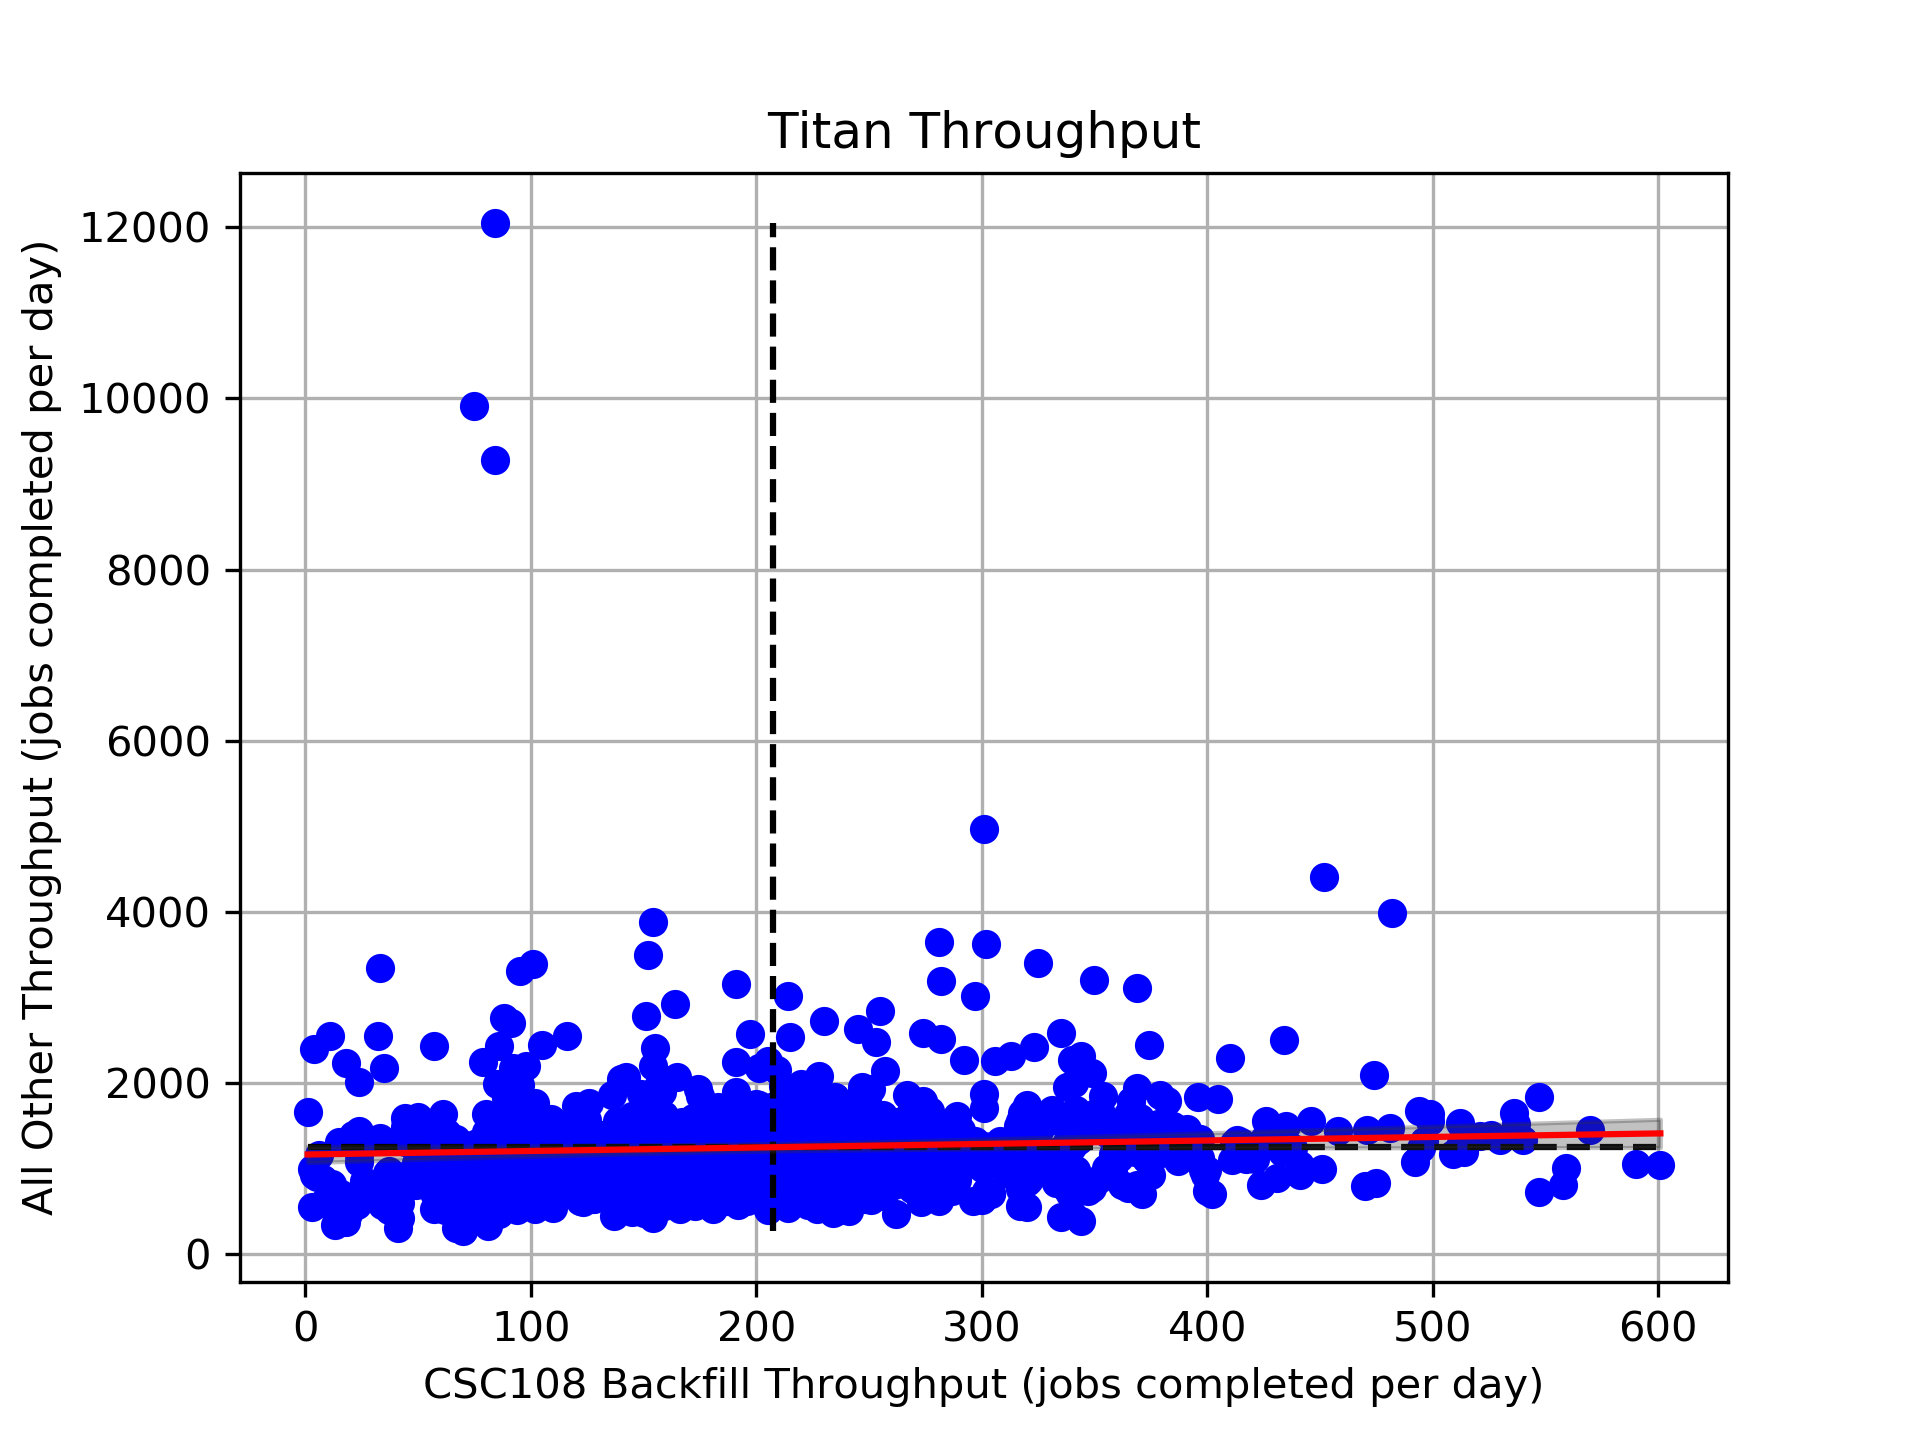
\includegraphics[width=0.4\textwidth]{images/linfit-throughput-all.png}}
  \subfloat[Bin 3\label{fig:throughput-bin3}]{
    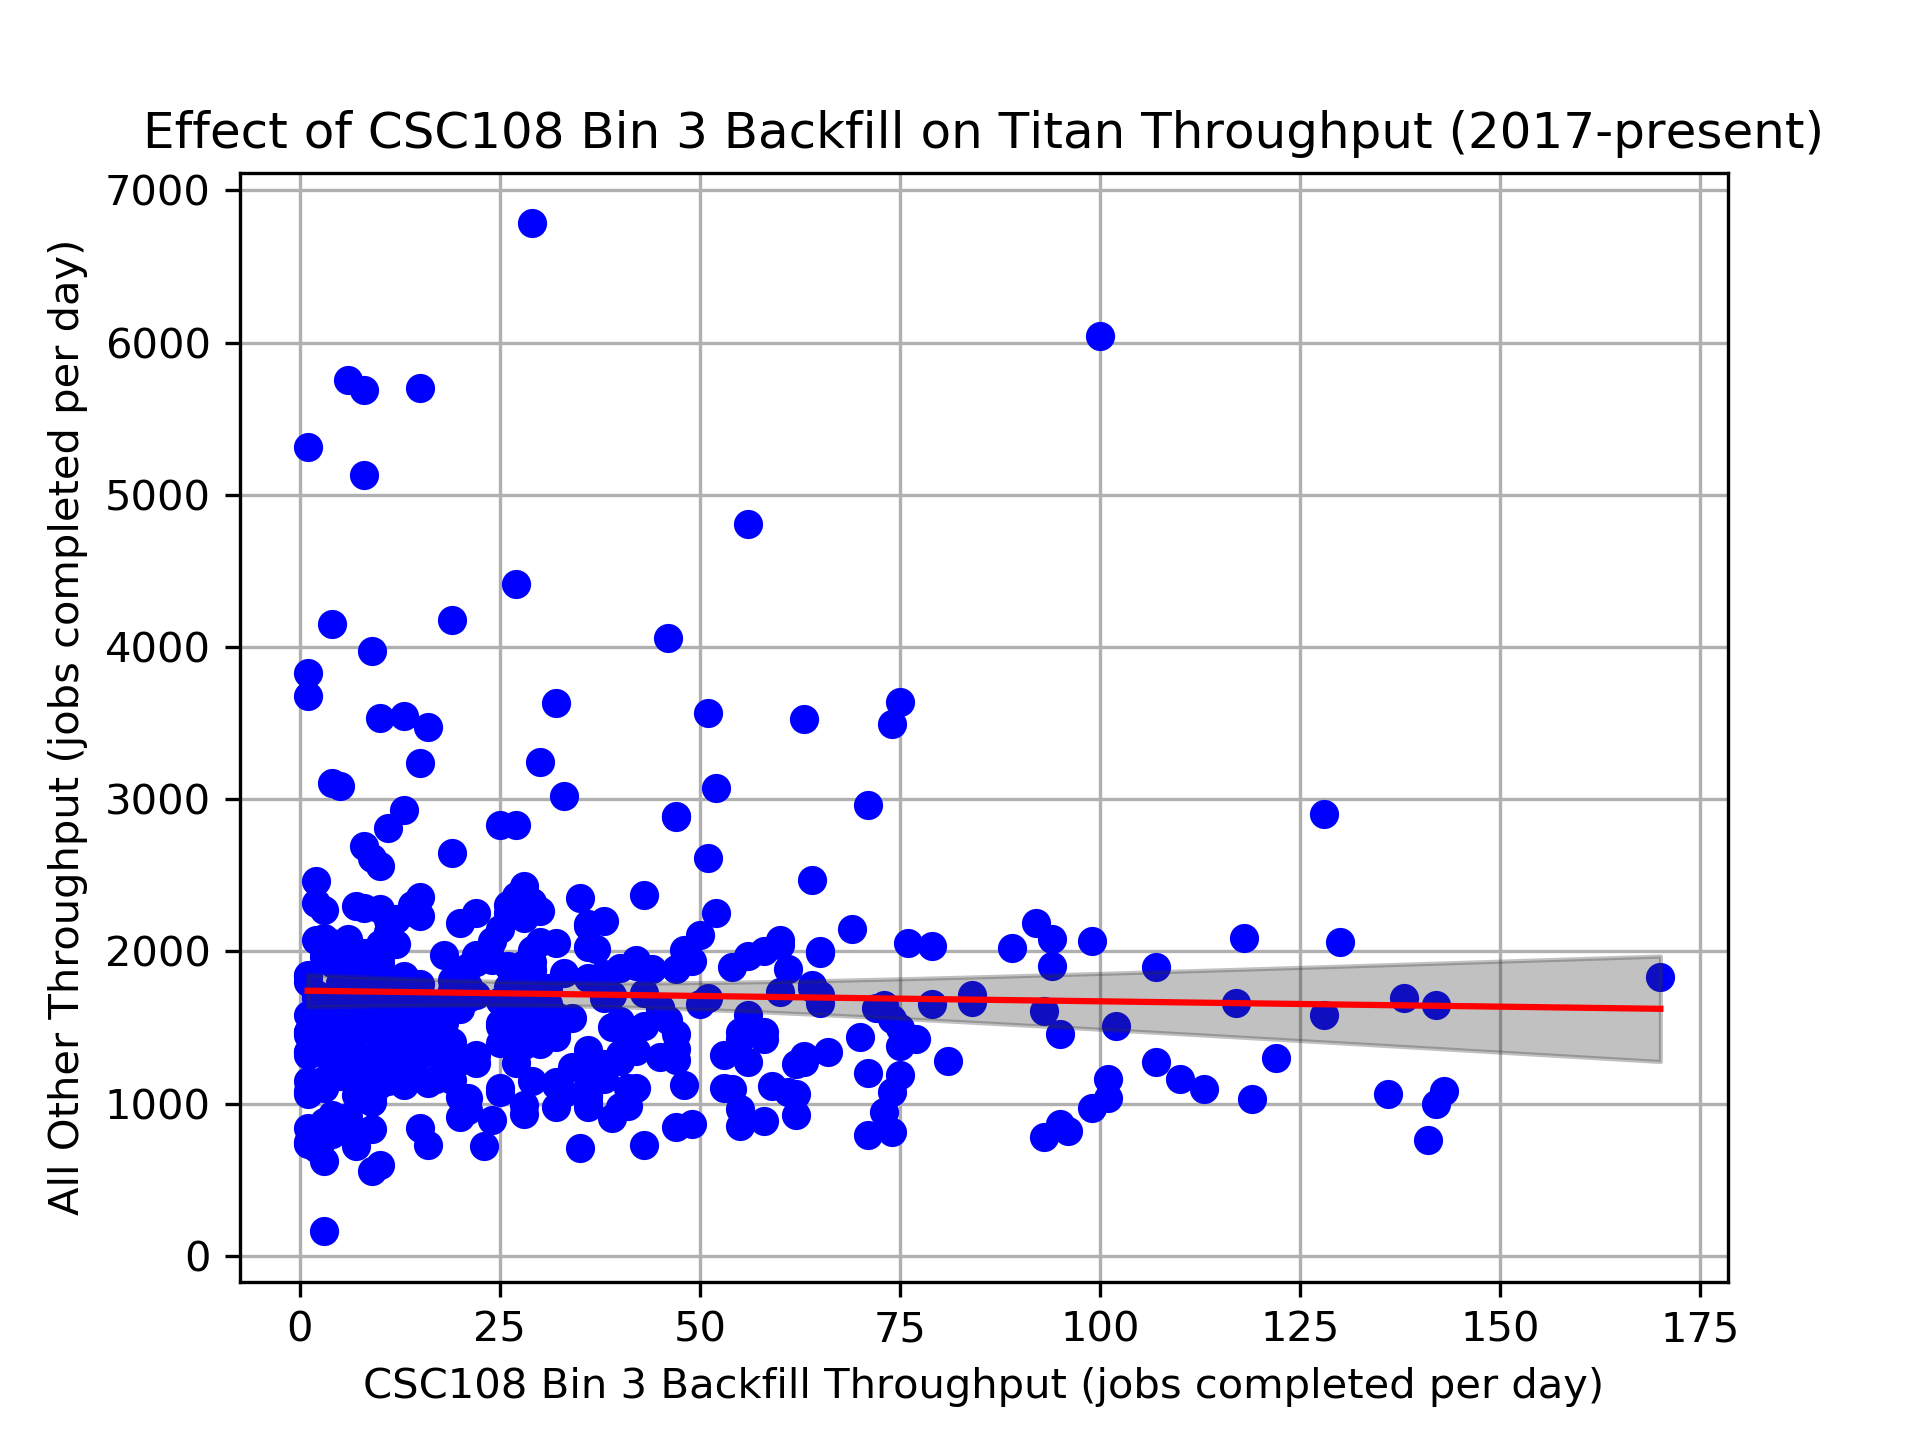
\includegraphics[width=0.4\textwidth]{images/linfit-throughput-bin3.png}}
  \vspace{1em}
  \subfloat[Bin 4\label{fig:throughput-bin4}]{
    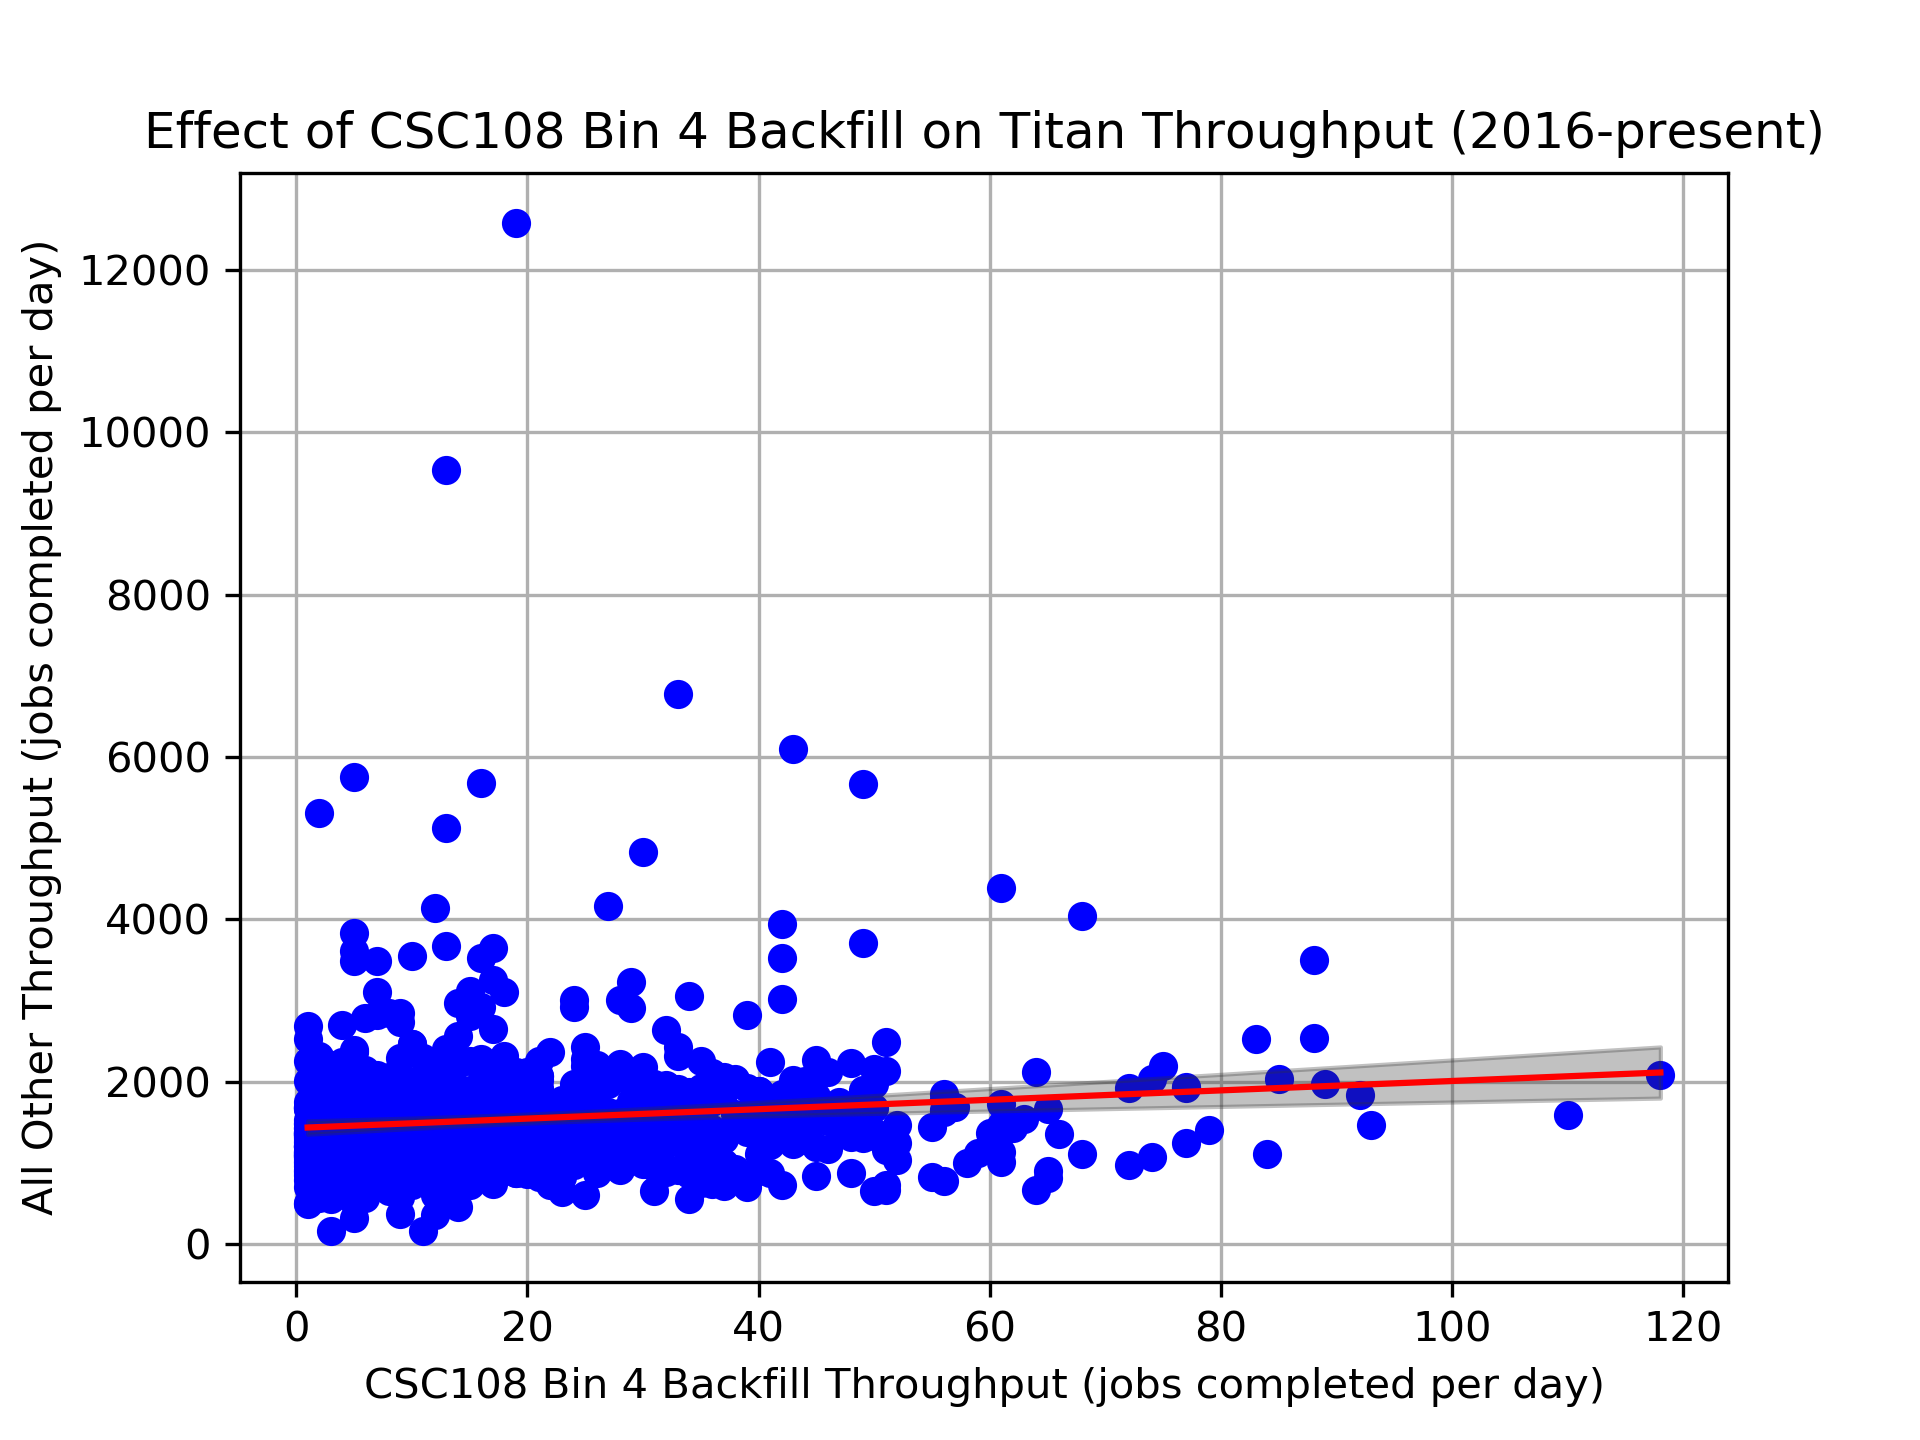
\includegraphics[width=0.4\textwidth]{images/linfit-throughput-bin4.png}}
  \subfloat[Bin 5\label{fig:throughput-bin5}]{
    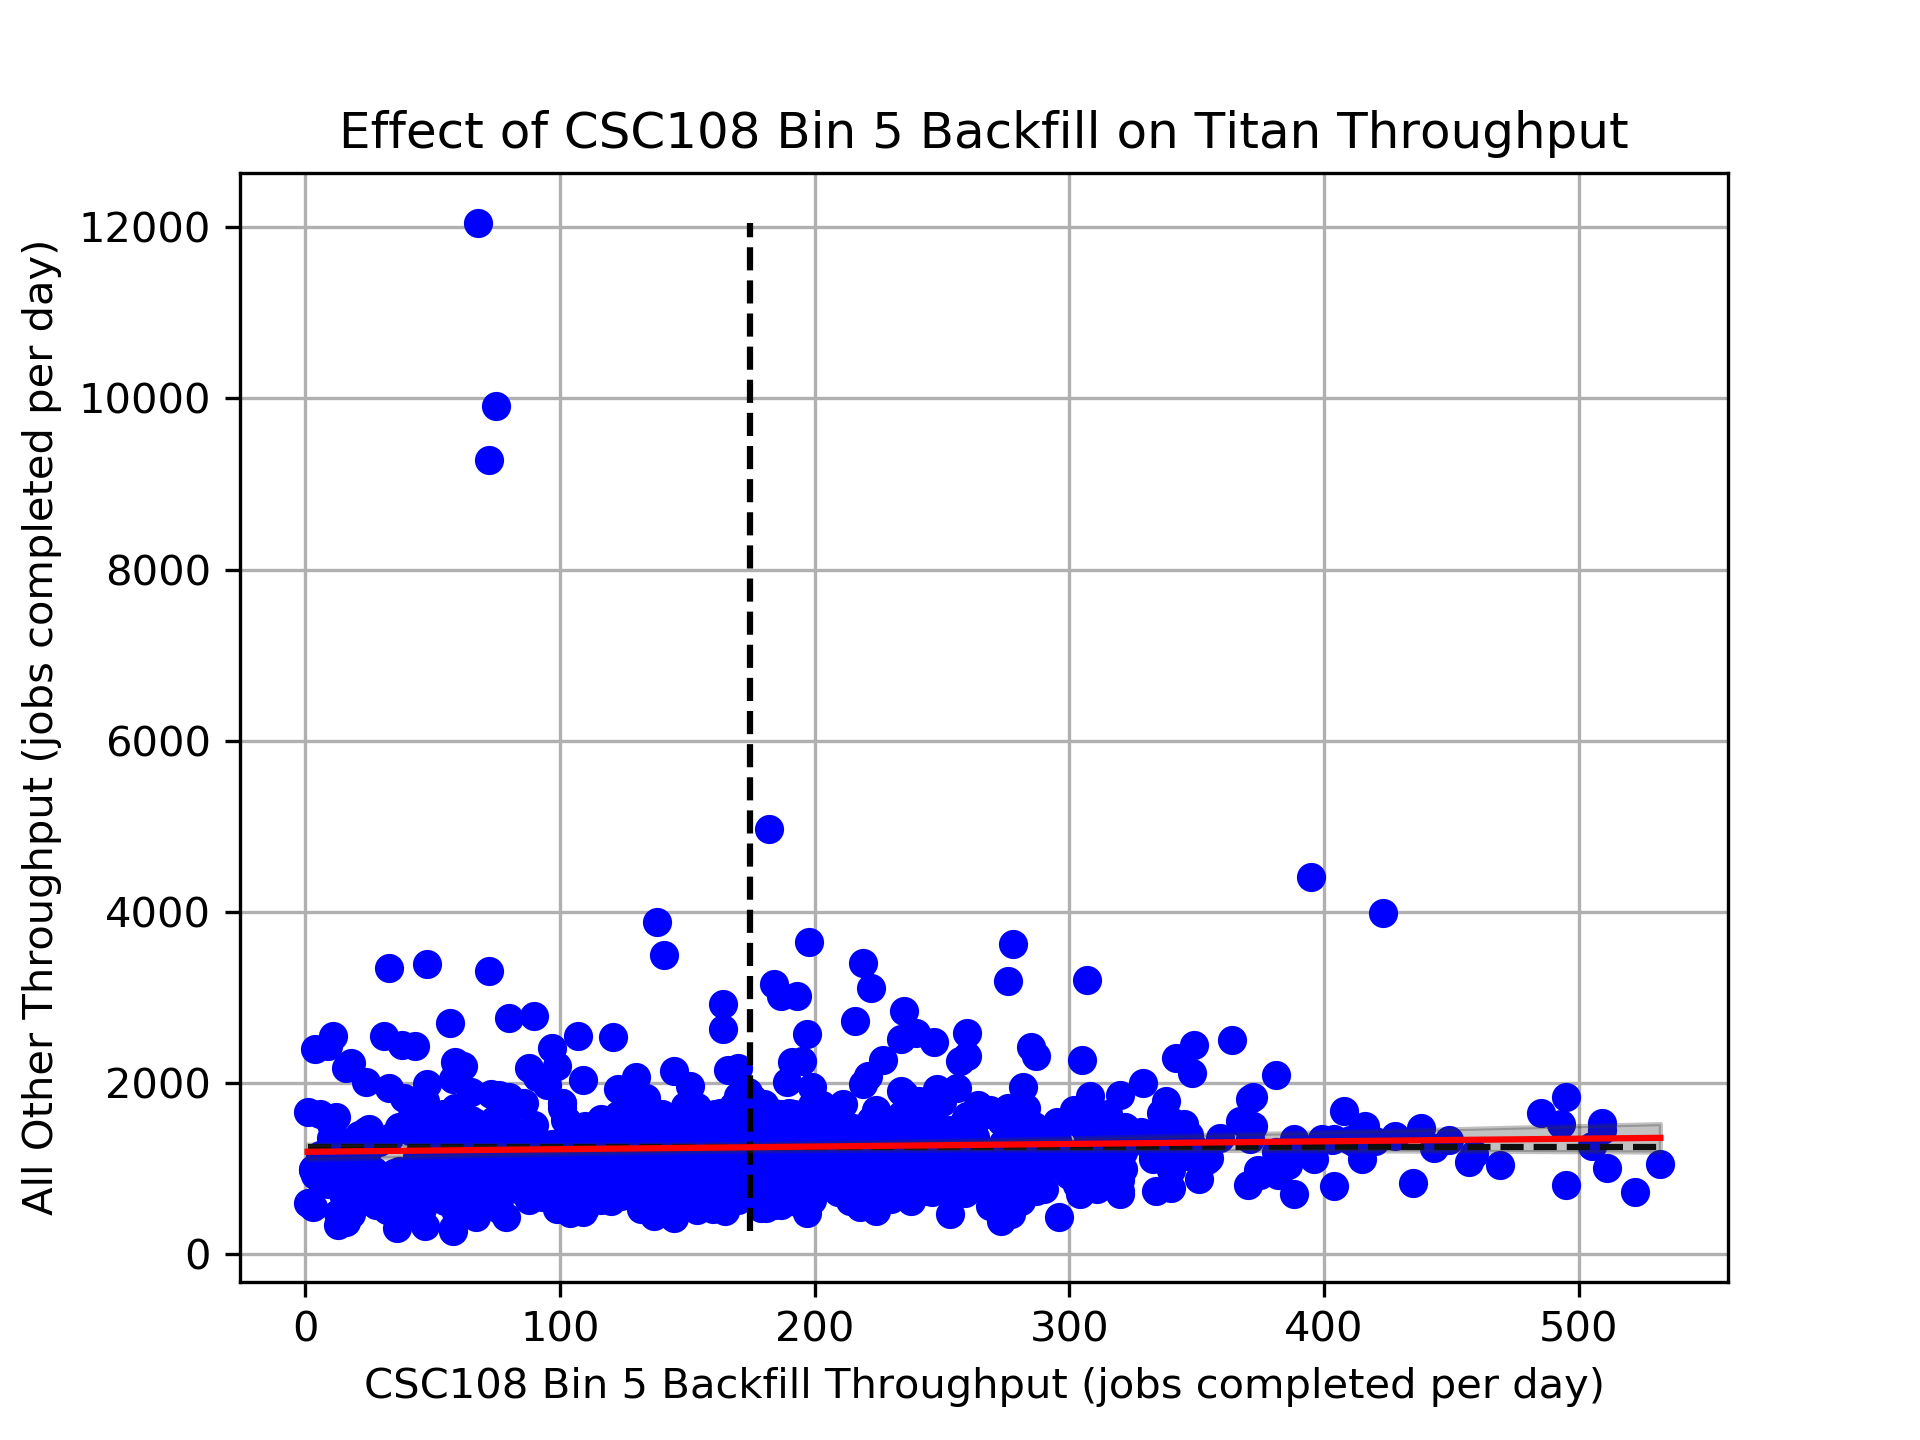
\includegraphics[width=0.4\textwidth]{images/linfit-throughput-bin5.png}}
  \caption{This figure demonstrates the relationship between CSC108 backfill
throughput and throughput of other projects on Titan, in terms of jobs
completed per day. Each blue point represents one day. Each red line is an
Ordinary Least Squares (OLS) linear regression with parameters given in
Table~\ref{tab:throughput-params}. Each shaded gray area represents a 95\%
confidence region. Each horizontal dotted black line represents the mean number
of jobs completed on Titan every day by projects other than CSC108, and the
vertical dotted black line represents the mean number of jobs completed every
day by CSC108's use of backfill opportunity.}
\end{figure*}

% For tables use
\begin{table}
% table caption is above the table
\caption{The table contains the parameter values for the Ordinary Least Squares
(OLS) linear regression models regarding throughput. The first column
corresponds to the figure depicting the model, and the second column
corresponds to the OLCF bin number, as defined in Table~\ref{tab:olcf-bins}.
The second and third columns correspond the coefficients $\beta_1$ and
$\beta_0$ in the model $y = \beta_{1}x + \beta_0$.}
\label{tab:throughput-params}       % Give a unique label
% For LaTeX tables use
\begin{tabular}{ccrrr}
\hline\noalign{\smallskip}
Figure & OLCF Bin & Slope $\beta_1$  & Intercept $\beta_0$  &   $\text{R}^2$ \\
\noalign{\smallskip}\hline\noalign{\smallskip}
\ref{fig:throughput-all}    &   All &   0.4106  &   1164.2561   & 0.0040    \\
\ref{fig:throughput-bin3}   &   3   &   0.4419  &   1322.0784   & 0.0005    \\
\ref{fig:throughput-bin4}   &   4   &   1.9819  &   1211.3384   & 0.0027    \\
\ref{fig:throughput-bin5}   &   5   &   0.3072  &   1195.6684   & 0.0018    \\
\noalign{\smallskip}\hline
\end{tabular}
\end{table}
%%%

%%%
% UTILIZATION FIGURES AS SUBFIGURES
%%%
\begin{figure*}
  \subfloat[All\label{fig:utilization-all}]{
    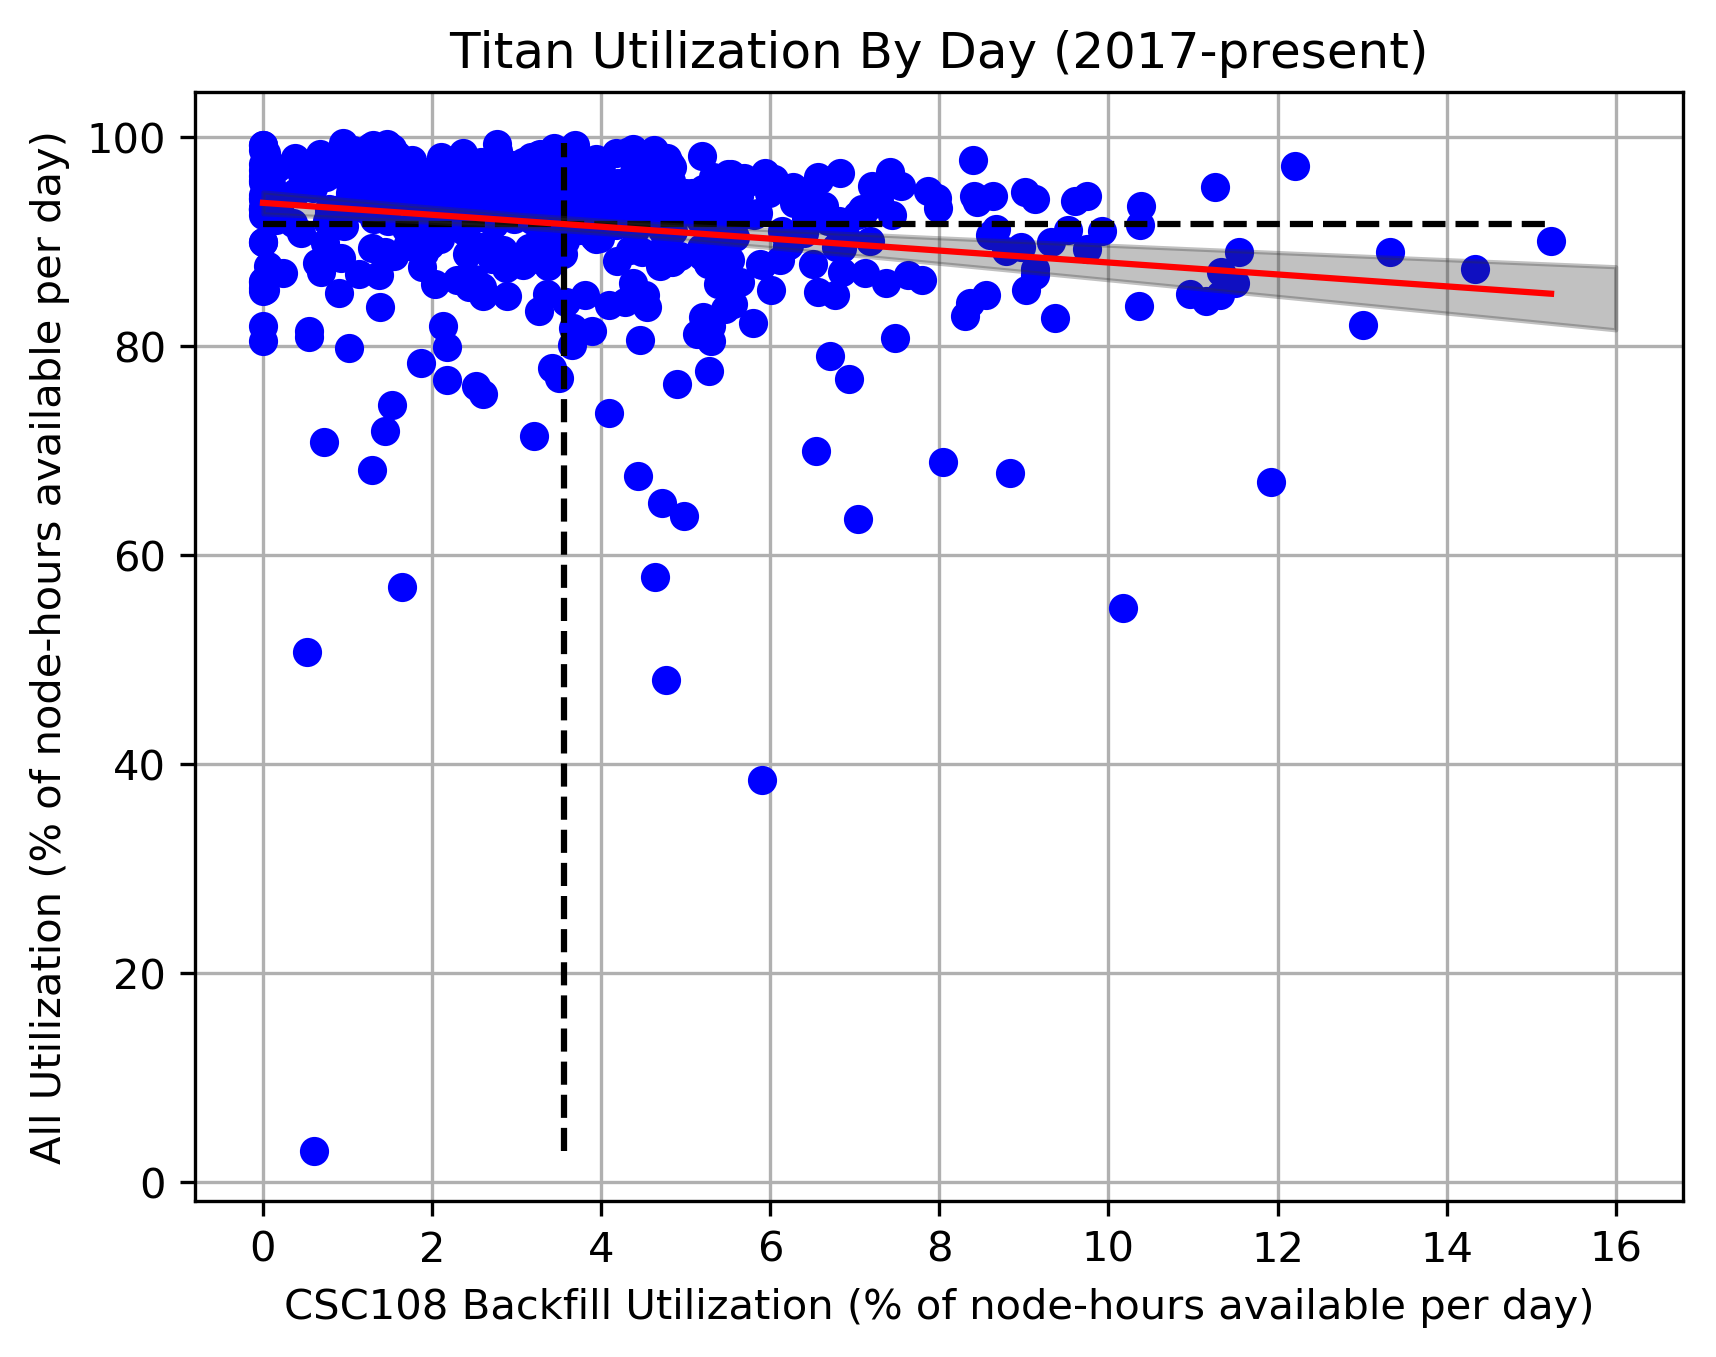
\includegraphics[width=0.4\textwidth]{images/linfit-utilization-by-true-day-all.png}}
  \subfloat[Bin 3\label{fig:utilization-bin3}]{
    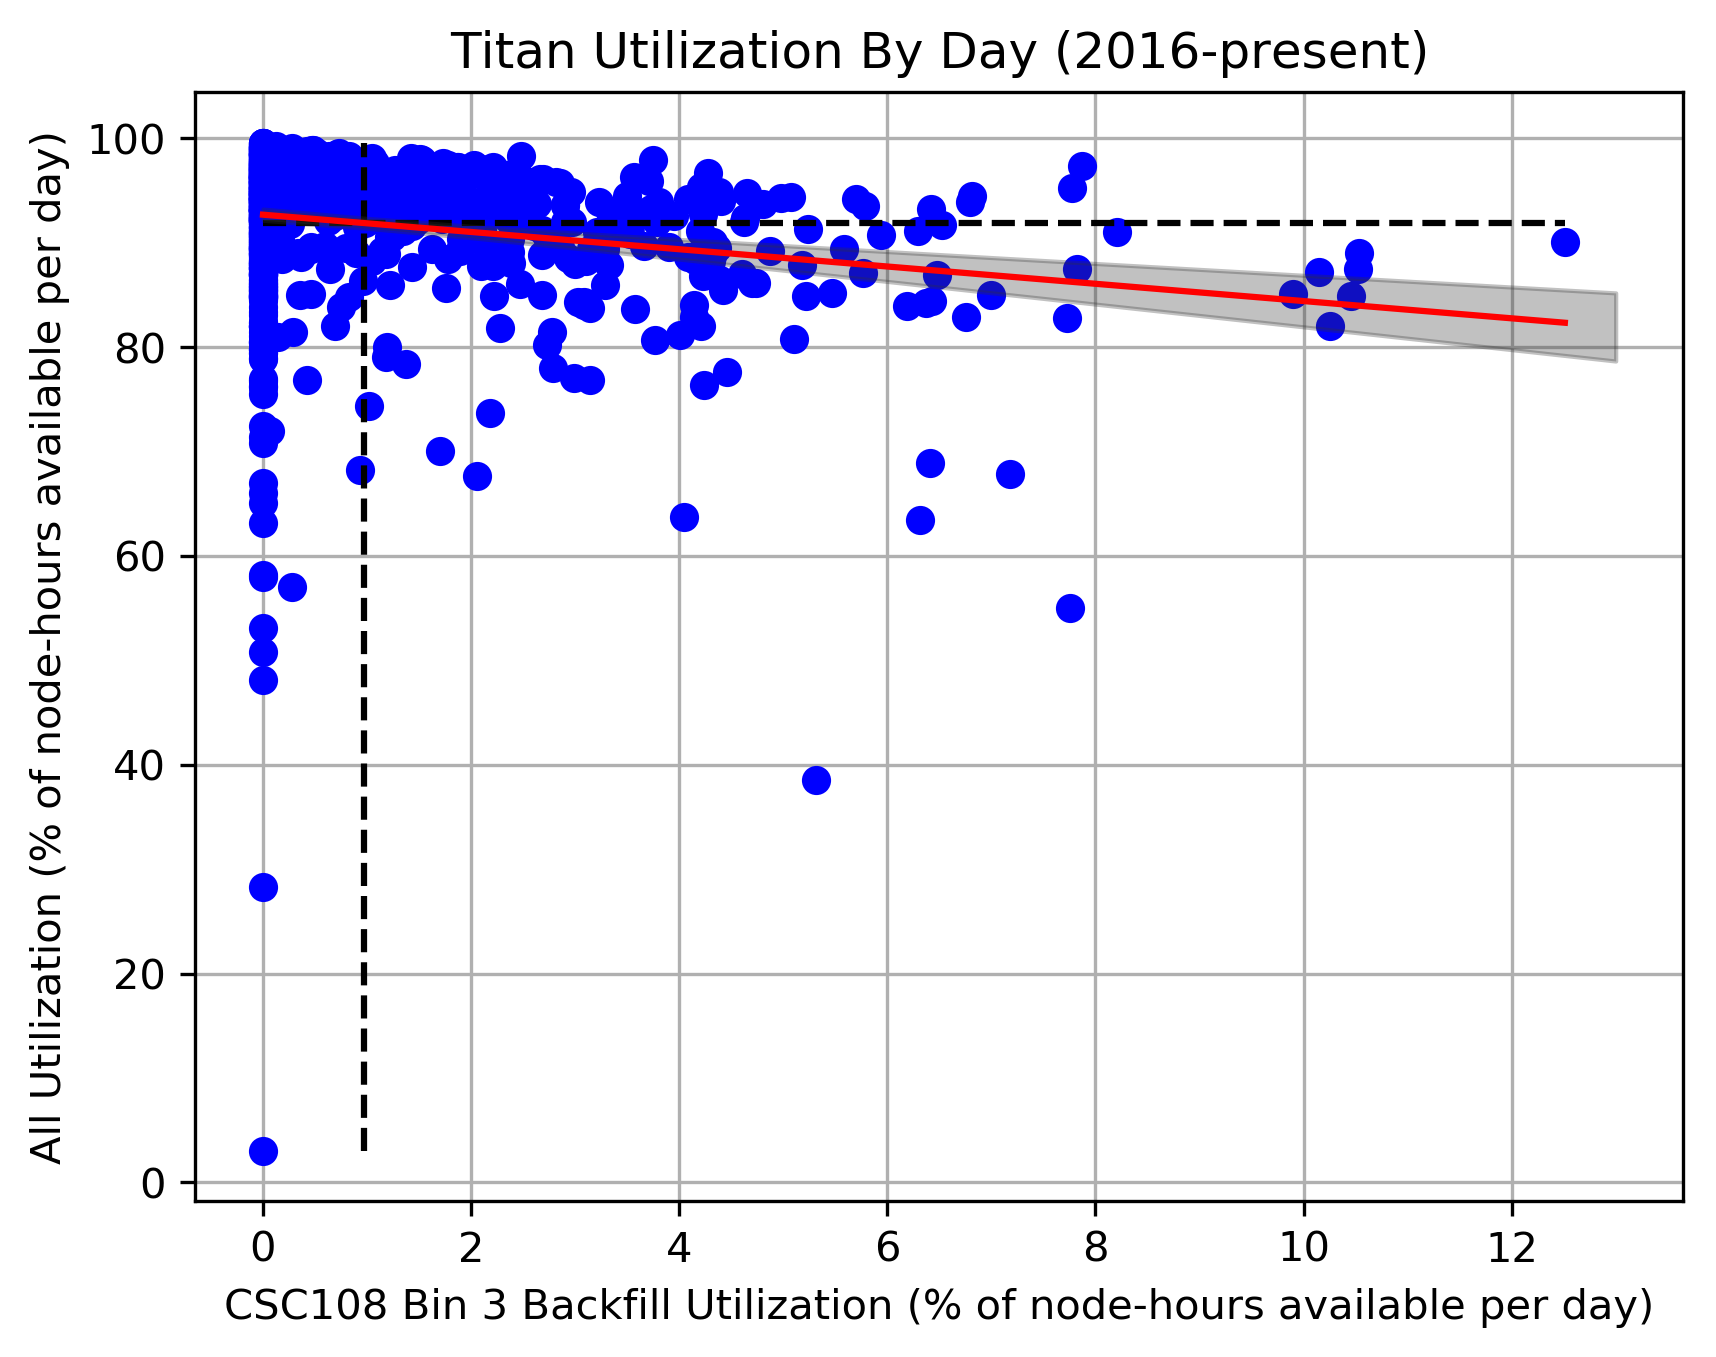
\includegraphics[width=0.4\textwidth]{images/linfit-utilization-by-true-day-bin3.png}}
  \vspace{1em}
  \subfloat[Bin 4\label{fig:utilization-bin4}]{
    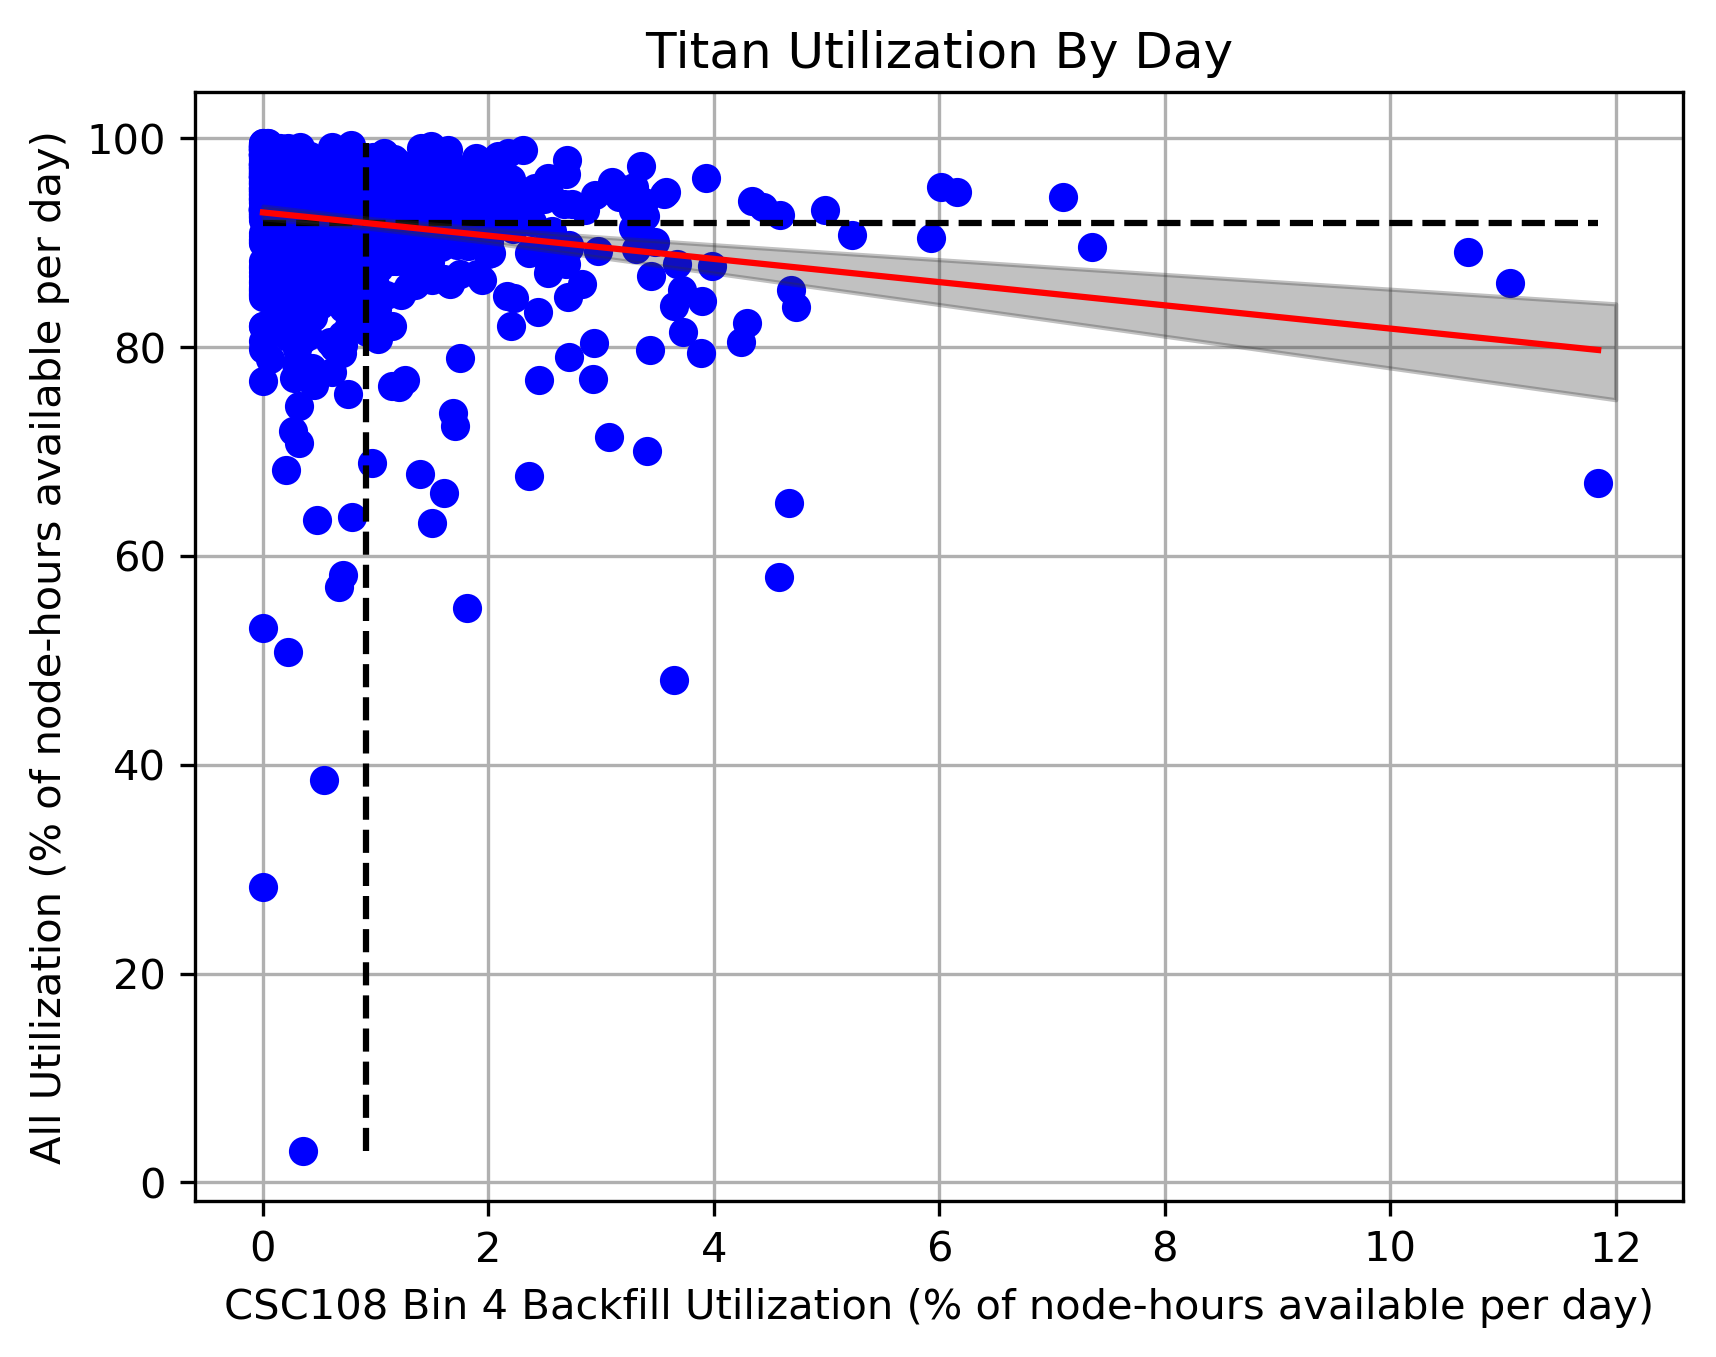
\includegraphics[width=0.4\textwidth]{images/linfit-utilization-by-true-day-bin4.png}}
  \subfloat[Bin 5\label{fig:utilization-bin5}]{
    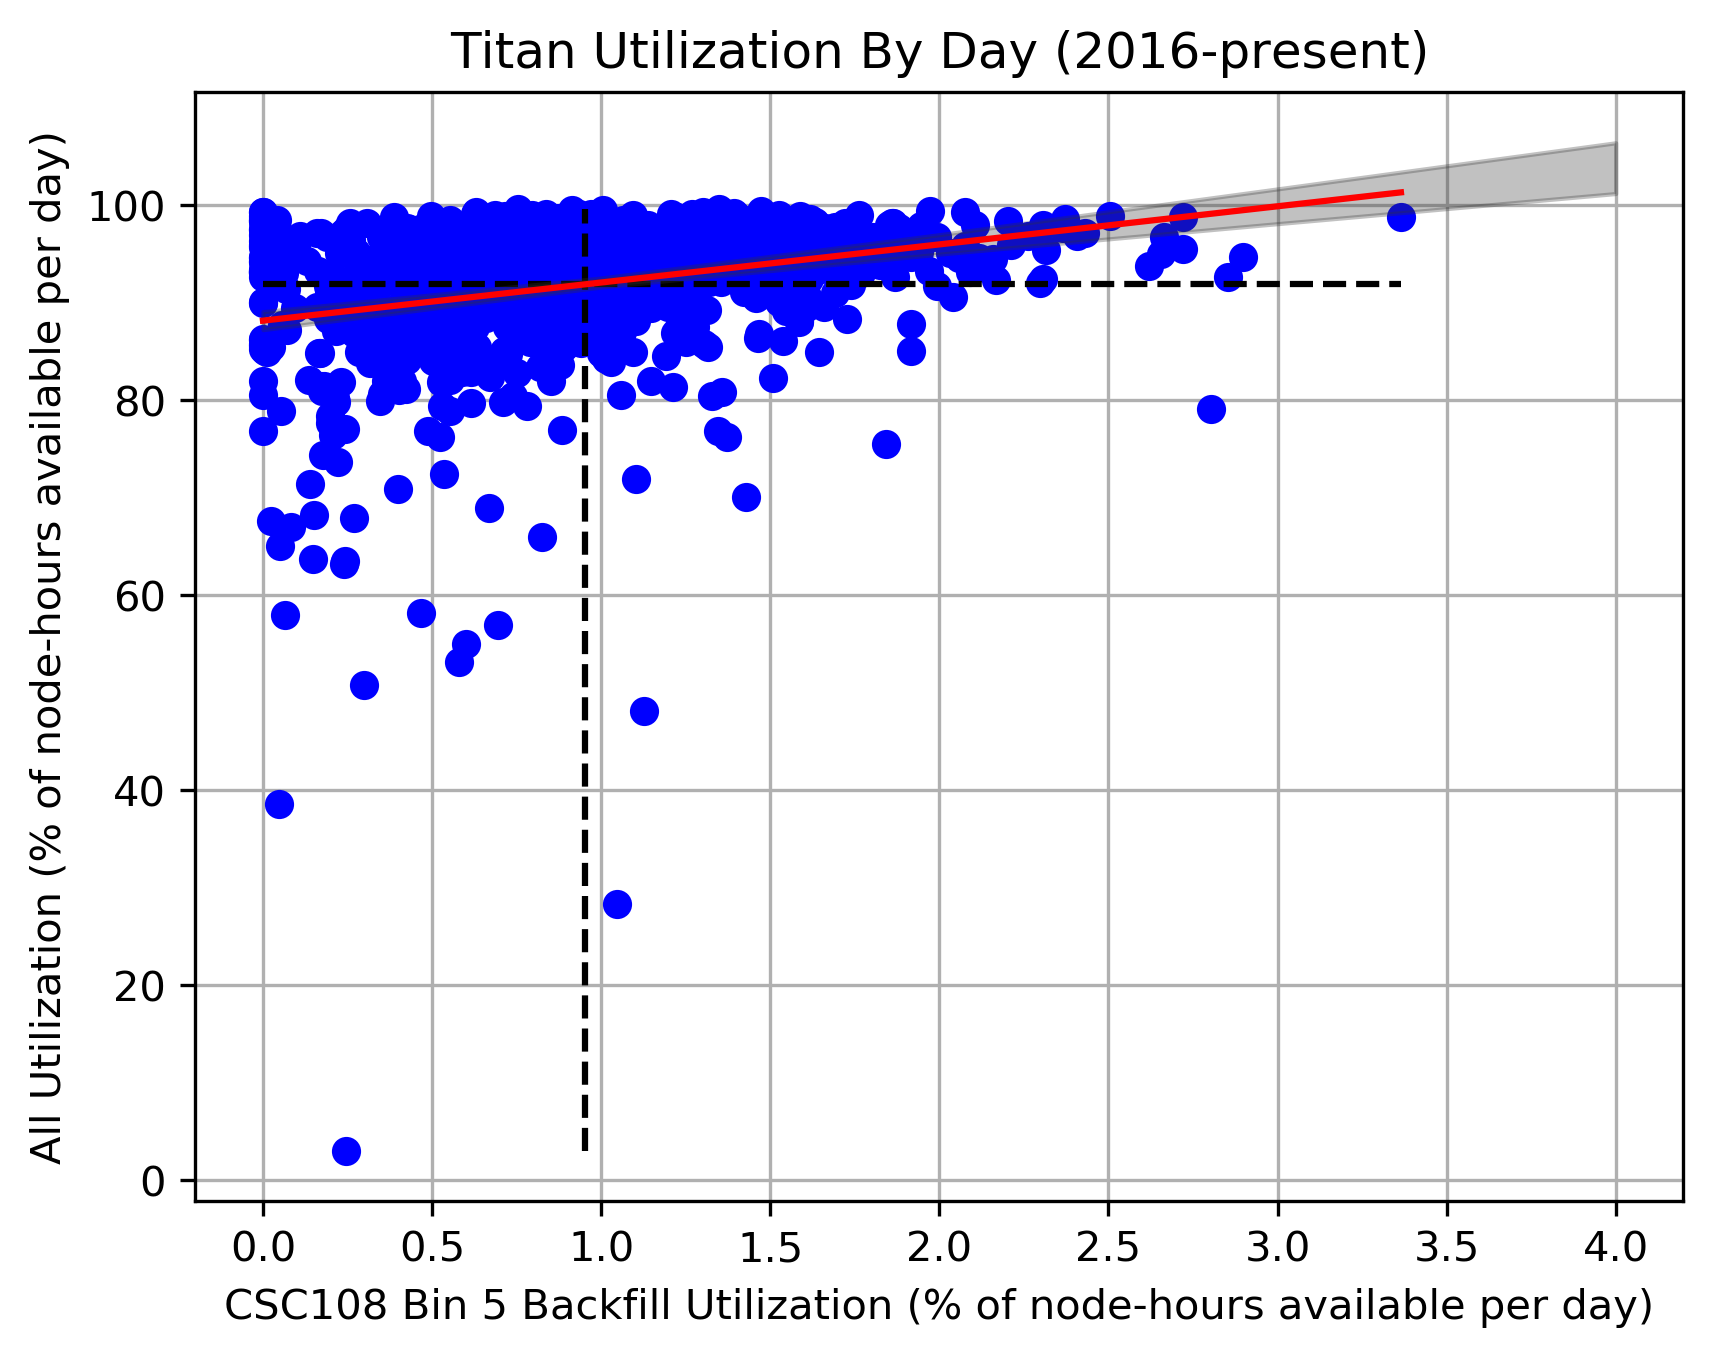
\includegraphics[width=0.4\textwidth]{images/linfit-utilization-by-true-day-bin5.png}}
  \caption{This figure demonstrates the relationship between CSC108 backfill
utilization and overall utilization on Titan, as percentages of available
node-hours each day. Each blue point represents one day. Each red line is an
Ordinary Least Squares (OLS) linear regression with parameters given in
Table~\ref{tab:utilization-params}. Each shaded gray area represents a 95\%
confidence regions. Each horizontal dotted black line represents the mean
utilization every day on Titan, and each vertical dotted black line represents
the mean utilization of backfill opportunity every day by CSC108.}
\end{figure*}

% For tables use
\begin{table}
% table caption is above the table
\caption{The table contains the parameter values for the Ordinary Least Squares
(OLS) linear regression models regarding utilization. The first column
corresponds to the figure depicting the model, and the second column
corresponds to the OLCF bin number, as defined in Table~\ref{tab:olcf-bins}.
The second and third columns correspond the coefficients $\beta_1$ and
$\beta_0$ in the model $y = \beta_{1}x + \beta_0$.}
\label{tab:utilization-params}       % Give a unique label
% For LaTeX tables use
\begin{tabular}{ccrrr}
\hline\noalign{\smallskip}
Figure  & OLCF Bin & Slope $\beta_1$  & Intercept $\beta_0$  &  $\text{R}^2$ \\
\noalign{\smallskip}\hline\noalign{\smallskip}
\ref{fig:utilization-all}    &   All &  -0.5258 &   93.3404     &   0.0330  \\
\ref{fig:utilization-bin3}   &   3   &  -1.0977 &   94.0609     &   0.1359  \\
\ref{fig:utilization-bin4}   &   4   &  -1.1472 &   92.7870     &   0.0378  \\
\ref{fig:utilization-bin5}   &   5   &   4.3328 &   87.5839     &   0.1046  \\
\noalign{\smallskip}\hline
\end{tabular}
\end{table}
%%%

The plots shown in Figures~\ref{fig:throughput-all}, \ref{fig:throughput-bin3},
\ref{fig:throughput-bin4}, and \ref{fig:throughput-bin5} visually suggest that
CSC108 has little to no effect on other projects' throughputs, but the numbers
in Table~\ref{tab:throughput-params} show that linear relationships explain
very little of the variability in the data. The $\text{R}^2$ values, which
represent goodness-of-fit on a scale of 0 to 1, are very close to 0, indicating
poor fit.

Similar problems exist for the utilization results, but they raise one very
interesting question. The plots shown in Figures~\ref{fig:utilization-all},
\ref{fig:utilization-bin3}, and \ref{fig:utilization-bin4} are all suggestive
of an inverse relationship, but \ref{fig:utilization-bin5} suggests a direct
relationship, by virtue of its positive slope. The $R^2$ values show that
linear relationships explain very little of the variability in the data,
however, as shown in Table~\ref{tab:utilization-params}, because the
$\text{R}^2$ values are very close to 0, on a scale of 0 to 1. Thus, there are
no simple linear relationships at work here, because the goodness-of-fit values
are consistently close to 0.
\jhanote{Previous paragraph is casual and not precise. Needs fixing.}
\seannote{Agreed. I took out judgmental language and moved the opinions to be
stored in the Summary section for now.}

%%%%%%%%%%%%%%%%%%%%%%%%%%%%%%%%%%%%%%%%%%%%%%%%%%%%%%%%%%%%%%%%%%%%%%%%%%%%%%%%
\subsection{Blocking probability}
\label{subsec:blocking-probability}

The previous subsection analyzed traces for correlations between global set of
all jobs on Titan and CSC108 jobs. Although a useful exercise, the results are
at best inconclusive due to intrinsic noisiness which makes discerning
correlations even harder. In this section, we  try to model the underlying
process with the objective of moving beyond correlations and inferring casual
relationships between CSC108 scheduling events and a measure of impact
(utilization, wait time or throughput).

We begin by defining a ``block'' which is an event that occurs when an job
submitted to the batch queue is stalled in the wait state even though there
might be sufficient resources to run that job. A block typically occurs due to
some other job(s) using resources, and therefore the otherwise eligible job
has been ``blocked'' by an already-running job. A blocking event is
interesting because it indicates interference between jobs and competition for
resources even in the presence of available resources. A systematic analysis
of CSC108 has the potential to determine its impact on non-CSC108 jobs.

The data used for this experiment include the same historical trace data used
in Section~\ref{subsec:rescheduling-study} and the daily availability
data for Titan used in Section~\ref{subsec:simple-linear-relationships}, but
this time are supplemented with live snapshot data of the system queue for
Titan. Snapshots were gathered by sampling live data from the Moab scheduler by
polling with Python scripts launched by cron jobs on a data transfer node.
These scripts recorded XML output from the ``showbf'' and ``showq'' commands
into files, and more cron jobs launched other Python scripts to import these
files' sample data into SQLite. These tables contain data about the exact state
of the queues at given times, including active jobs, blocked jobs, eligible
jobs, recently completed jobs, and system information such as active nodes and
available backfill opportunities. Then, experimental programs were written in
Python using the same libraries and database as the previous sections.

Formally, the definitions for a block and a blocking probability follow. Let
$C_i$ be the abstract resources in use by CSC108 at the $i^{\text{th}}$ sample
point in time, and let $U_i$ be the unused (idle) resources remaining on
Titan. We then define a boolean $B_i$ representing a ``block'' event to occur
if there exists at least one job at the $i^{\text{th}}$ sample point which
requests $(C_i + U_i)$ resources or less (when $C_i$ is non-zero). If there is
no job at $i^{\text{th}}$ which requests more than $(C_i + U_i)$ we say a
blocking event $B_i$  does not occur. Summing $B_i$ over all $i$ gives a count
of the number of blocking events that occur, and dividing that count by the
number of total sample points yields a quantity we call a ``blocking
probability''.

Informally, blocking probability represents the proportion of samples 
\jhanote{sample of what? time? intervals possibly better term?} in which a
block occurred. The idea here is that when blocking probability increases, it
indicates that the system is experiencing greater competition for its
resources. Blocking probability does not predict the probability that a
particular job will be blocked, but rather the probability that a given sample
will contain a block.

To apply this abstract model to a real data set, we have initially defined the
resources in one-dimensional ``spatial'' and ``temporal'' manners, by
considering only jobs' requested numbers of nodes in the former and only jobs'
requested wall times in the latter. An eligible job in the batch queue is said
to be spatially blocked when the job’s number of requested nodes is too large
to fit within the nodes available through backfill opportunity, so that the job
must wait to run. Similarly, an eligible job in the batch queue is said to be
temporally blocked when the job’s requested wall time is too long to fit within
the duration available through backfill opportunity. Similarly, a job is said
to be blocked ``due to CSC108'' if at least one job which was blocked would no
longer be blocked if CSC108's jobs were removed. Thus, a job is only said to be
blocked due to CSC108 if it requests resources with are greater than $U_i$ but
less than $(C_i + U_i)$. Figures
\ref{fig:spatial-blocking-by-month} and \ref{fig:temporal-blocking-by-month}
demonstrate how spatial and temporal blocking probabilities vary from month to
month, and Figure~\ref{fig:spatial-vs-temporal} shows that the two quantities
relate to each other in an intuitive way, namely, that time periods of greater
spatial blocking often correspond to time periods of greater temporal blocking
as well.

%%%
% WAIT TIMES AS SUBFIGURES
\begin{figure*}
  \subfloat[Spatial blocking\label{fig:spatial-blocking-by-month}]{
    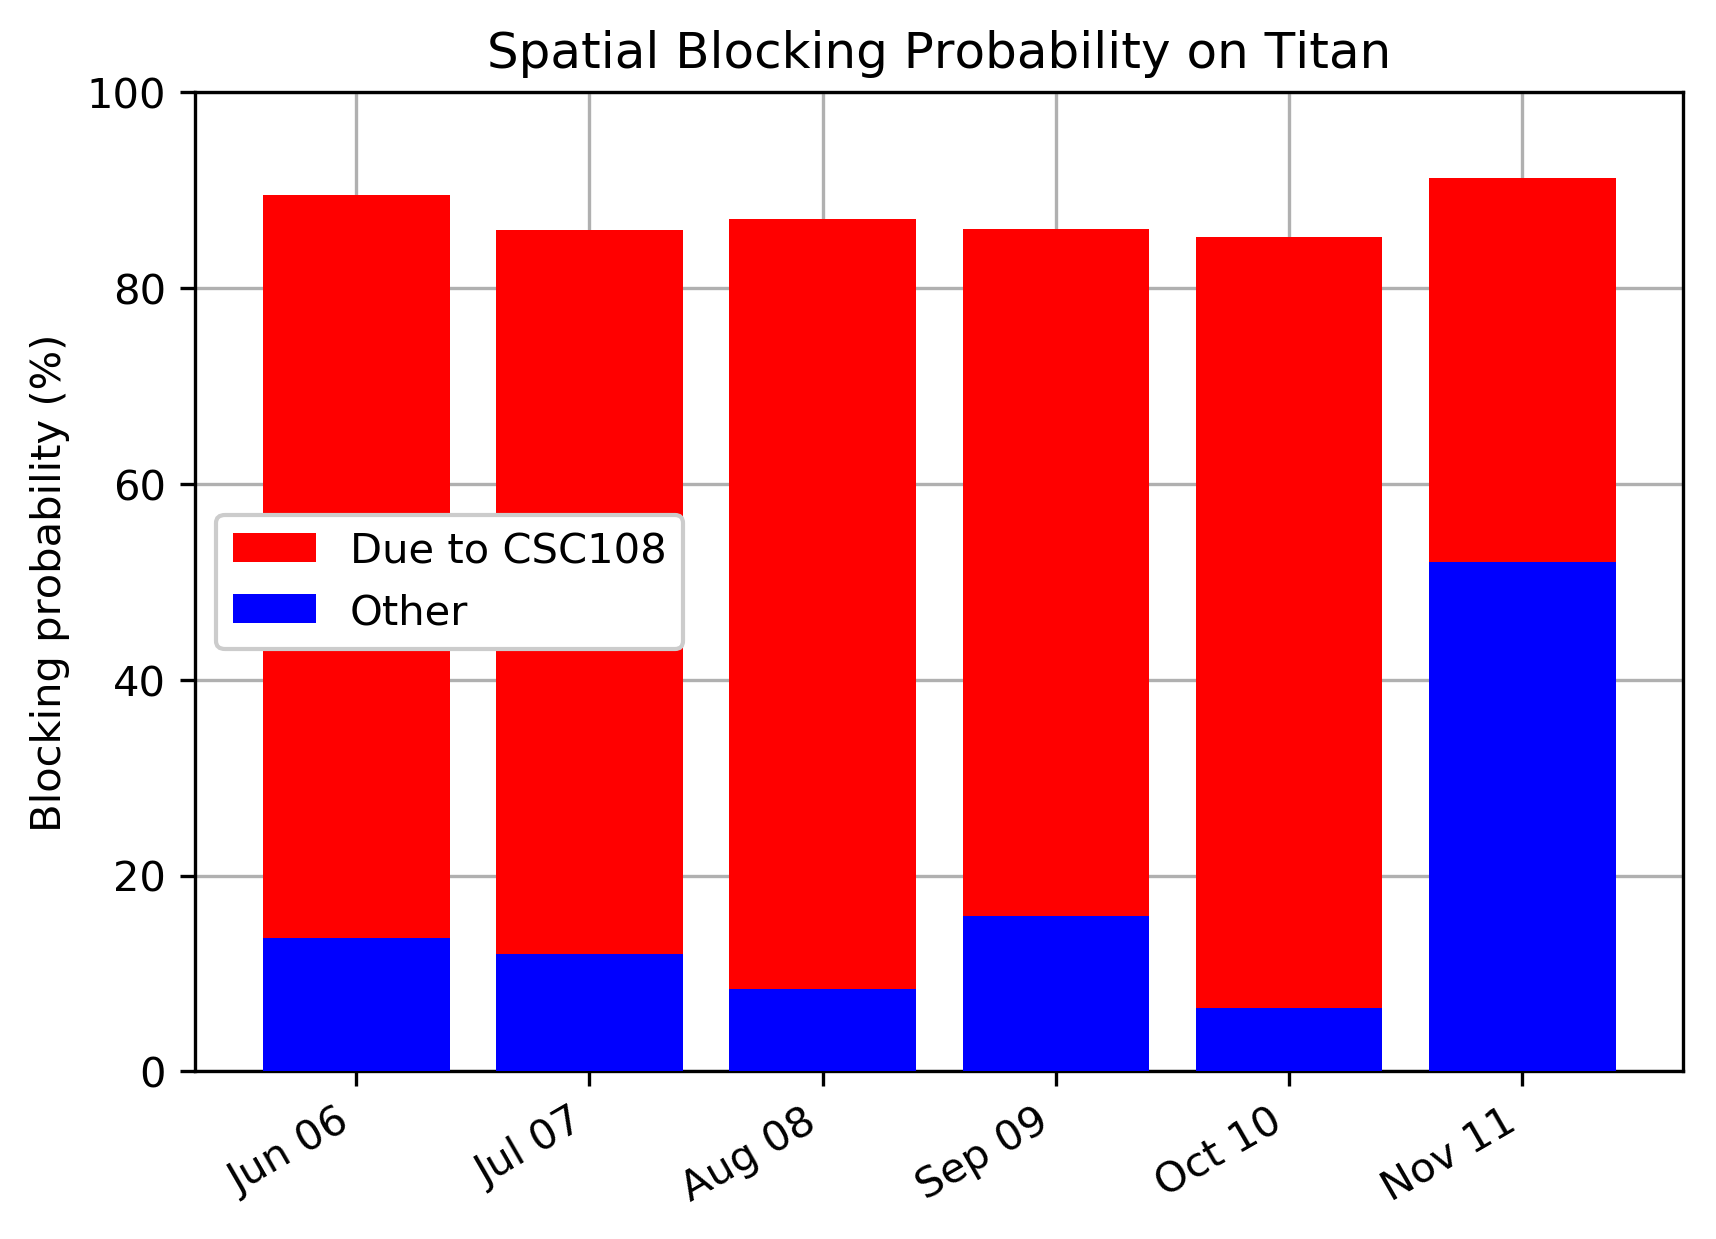
\includegraphics[width=0.4\textwidth]{images/barplot-spatial-blocking-by-month.png}}
  \subfloat[Temporal blocking\label{fig:temporal-blocking-by-month}]{
    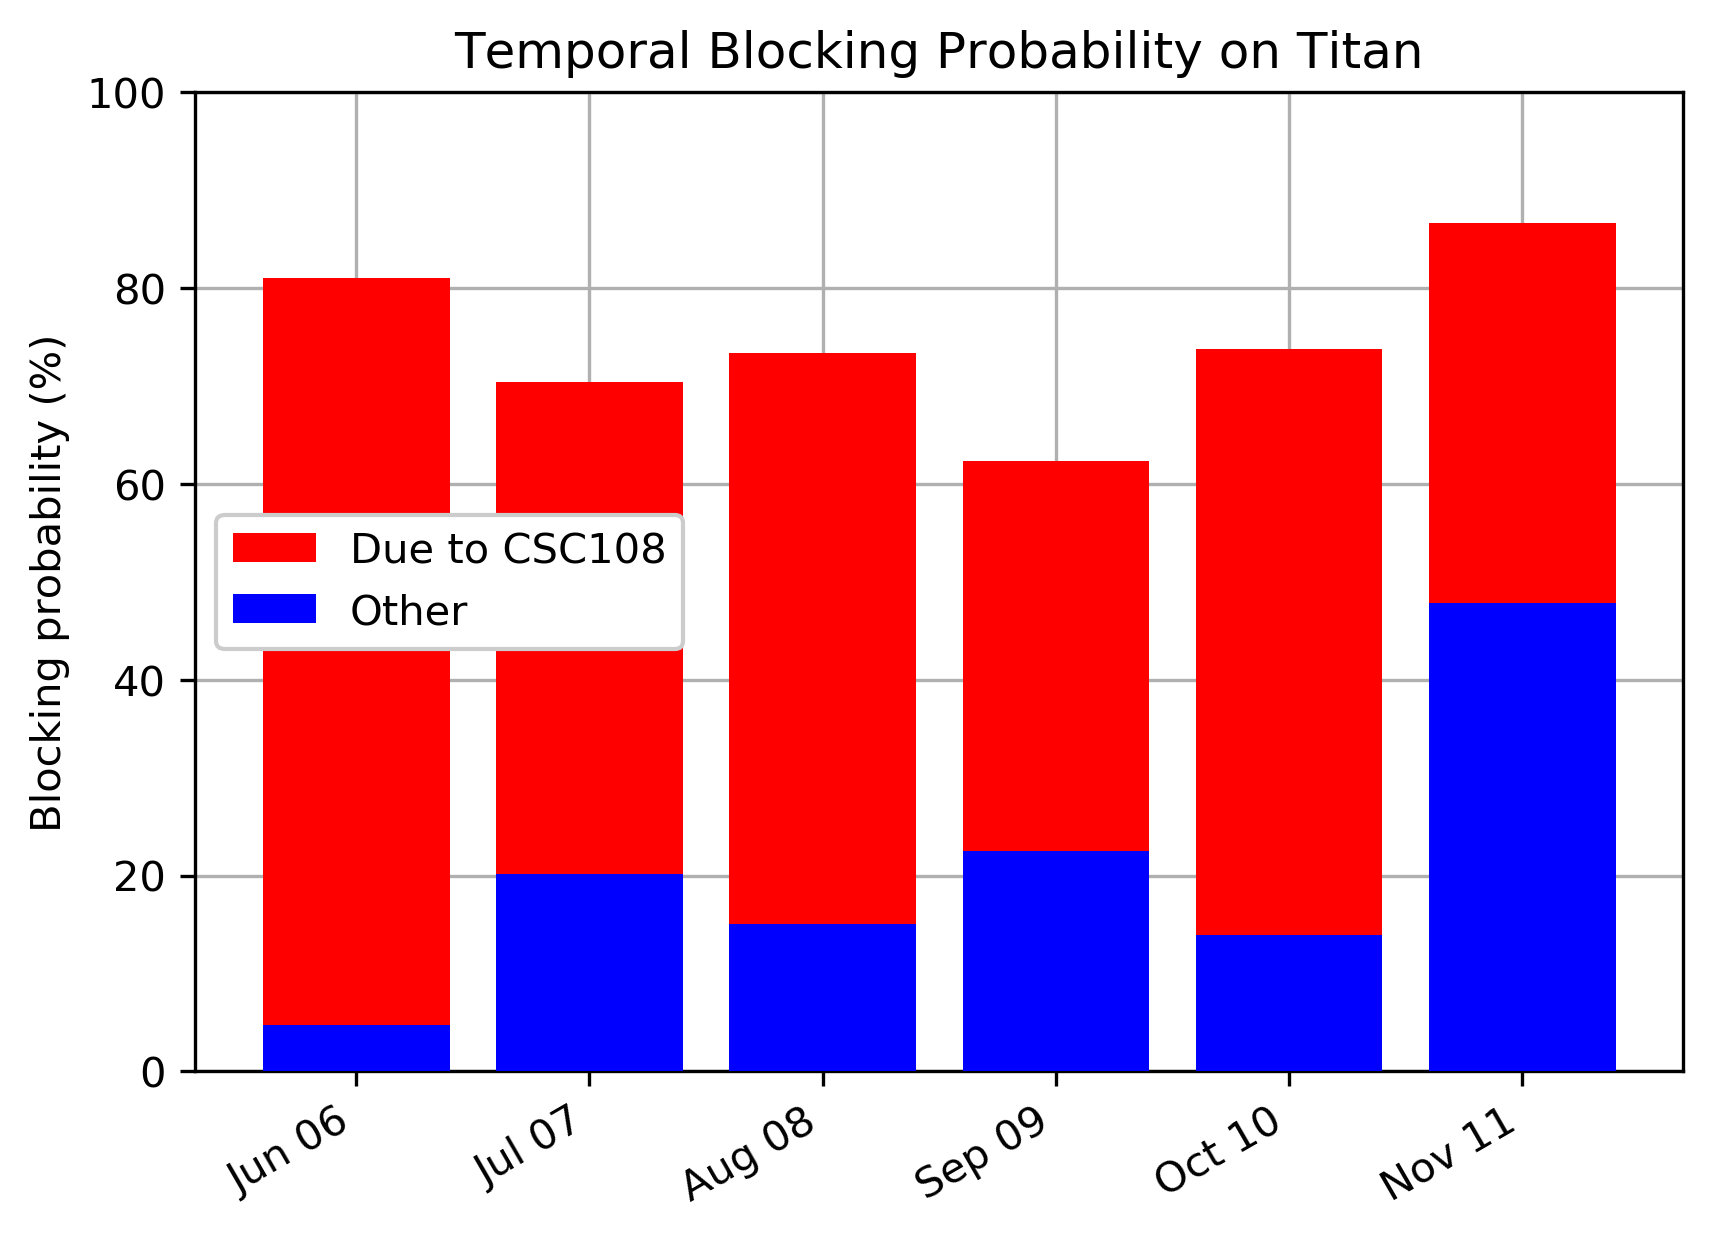
\includegraphics[width=0.4\textwidth]{images/barplot-temporal-blocking-by-month.png}}
  \caption{These plots depict the spatial and temporal blocking probabilities
by month for samples in which CSC108 was actively utilizing backfill
opportunity. The total height of the bars indicates the blocking probability
for the month, which is the proportion of samples in which at least one
eligible job was blocked. The red region indicates the percentage of samples in
which at least one eligible job would no longer be blocked if CSC108's jobs
were removed.}
\end{figure*}

% For two-column wide figures use
\begin{figure*}
% Use the relevant command to insert your figure file.
% For example, with the graphicx package use
  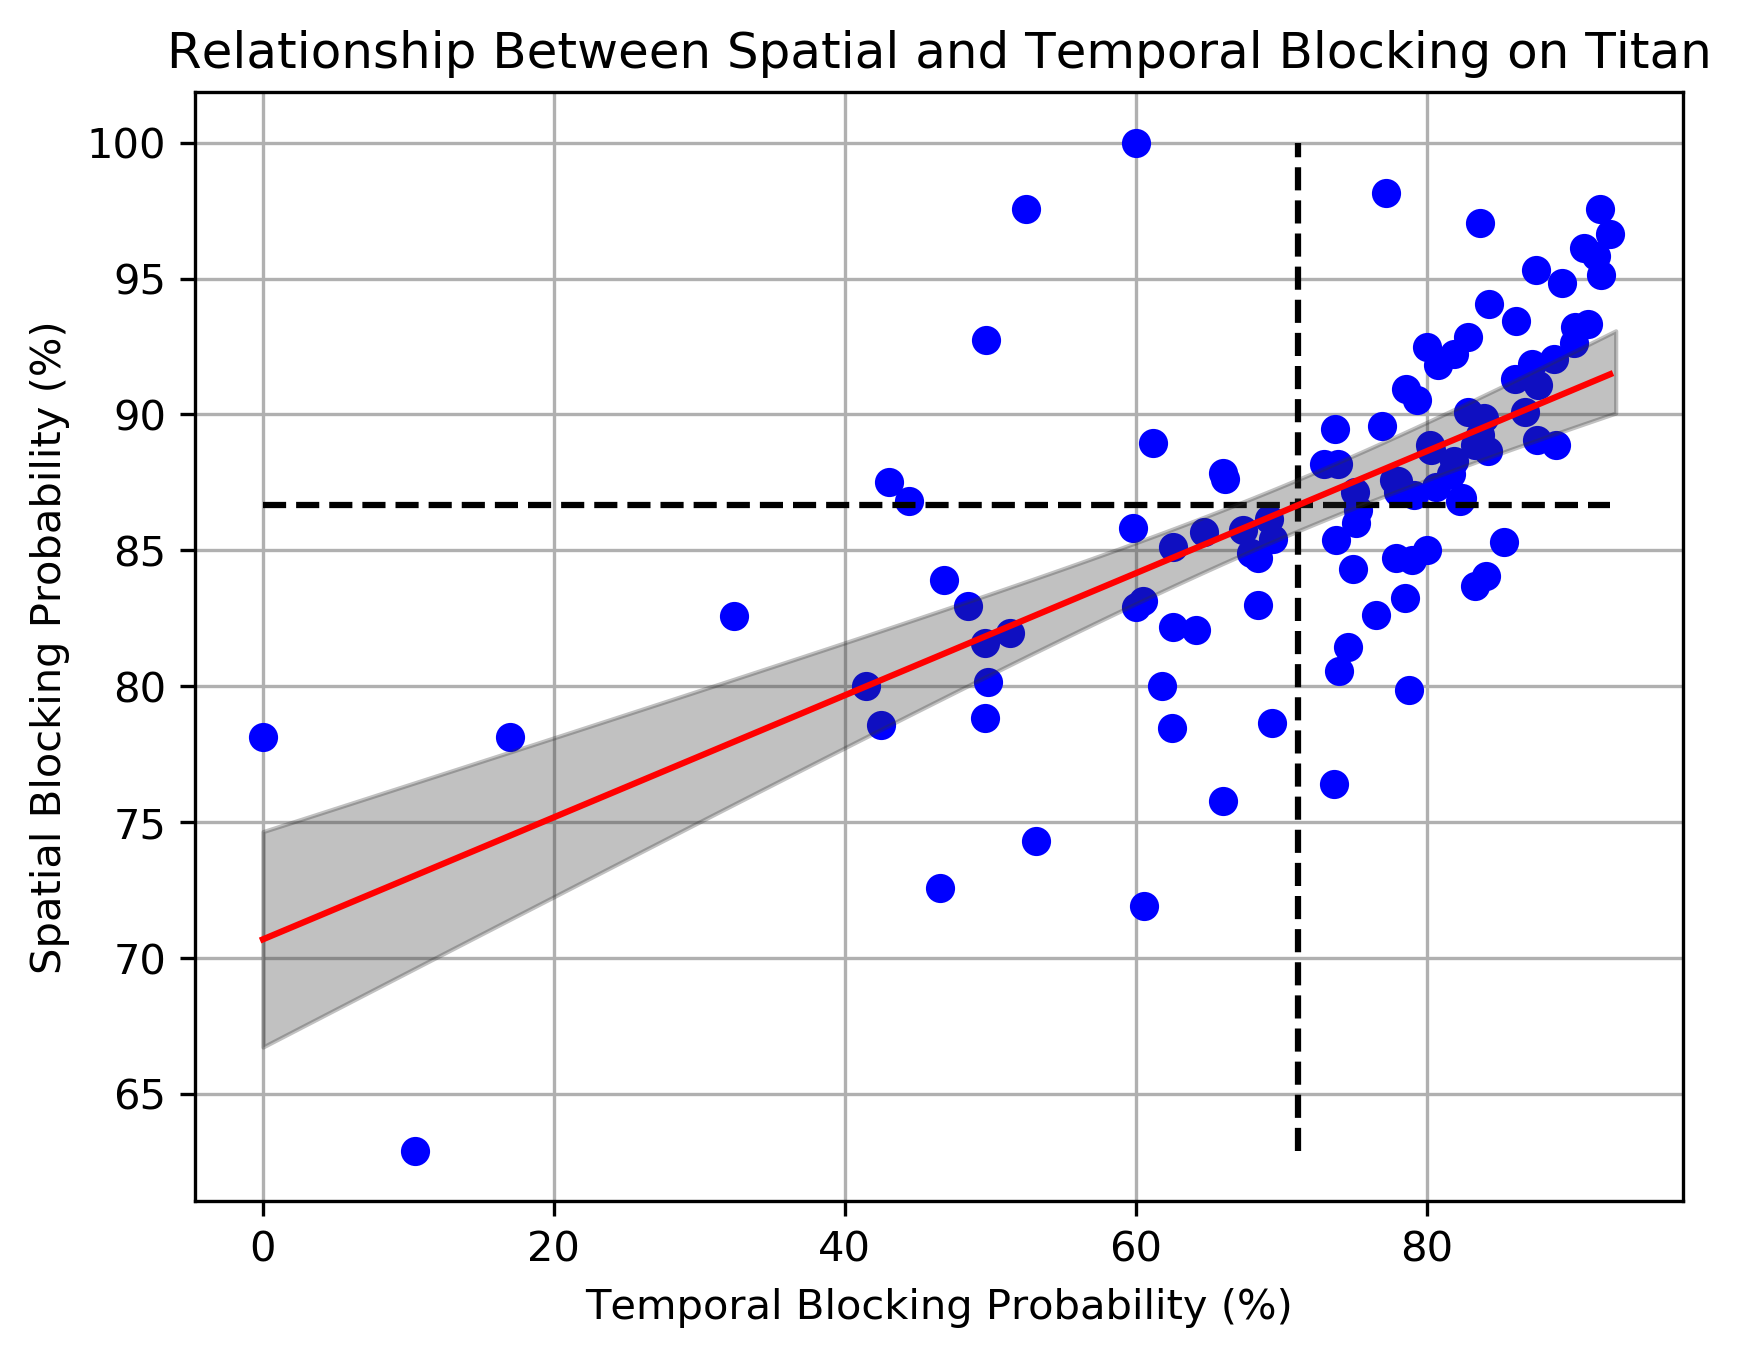
\includegraphics[width=0.75\textwidth]{images/linfit-spatial-vs-temporal-by-day.png}
% figure caption is below the figure
\caption{This figure demonstrates the relationship between spatial and temporal
blocking probabilities. Each blue point represents one day. The red line is an
Ordinary Least Squares (OLS) linear regression ($y = \beta_{1}x + \beta_0$)
with a slope $\beta_1$ of 0.2503 and an intercept $\beta_0$ of 68.7731. The
shaded gray areas represent 95\% confidence regions. The horizontal dotted
black line represents the mean spatial blocking probability for all points, and
the vertical dotted black line represents the mean temporal blocking
probability for all points. The $\text{R}^2$ value is 0.4410.}
\label{fig:spatial-vs-temporal}
\end{figure*}
%%%

Three indicators of system performance were chosen this time, as well, to
assess the impact of CSC108 on Titan: wait times, throughput, and utilization.
In order to map wait time to a value that can be attributed to a day, wait time
was defined in terms of an average wait time. Average wait time was defined as
the total number of hours spent waiting during a given day, per job that
appeared on that day. For example, a job which was submitted one day but which
did not run until the next day would contribute part of its wait time to the
first day and the rest to the second day, and it would be considered to have
appeared on both days. Throughput was defined as the number of jobs completed
per day, as before. Utilization was also defined as before, as the percentage
of core hours consumed out of the total core hours available.

%%% WAIT TIMES STUFF

Having established the two measures of blocking probability and their
relationship to one another, we followed the same techniques used in
Section~\ref{subsec:simple-linear-relationships} to create best-fit lines with
95\% confidence intervals, to investigate the relationships between blocking
probabilities and wait times experienced by jobs on Titan. Figures
\ref{fig:wait-time-spatial-all} and \ref{fig:wait-time-temporal-all} illustrate
the effects of spatial and temporal blocking probability on wait times, and
Figures \ref{fig:wait-time-spatial-csc108} and
\ref{fig:wait-time-temporal-csc108} show how CSC108's contribution to blocking
impacts wait times. More specifically, in Figures
\ref{fig:wait-time-spatial-csc108} and \ref{fig:wait-time-temporal-csc108}, the
values used for the blocking probabilities correspond to the red regions in
Figures \ref{fig:spatial-blocking-by-month} and
\ref{fig:temporal-blocking-by-month}, which indicate the percentage of samples
in which at least one eligible job would no longer be blocked if CSC108 freed
its resources. The qualitative interpretation for the wait time plots is that,
as competition for resources increases on Titan, average wait times decrease,
but when competition with CSC108 for nodes increases, average wait times
increase. Unfortunately, the goodness-of-fit values are again very poor.

\begin{figure*}
  \subfloat[Spatial blocking\label{fig:wait-time-spatial-all}]{
    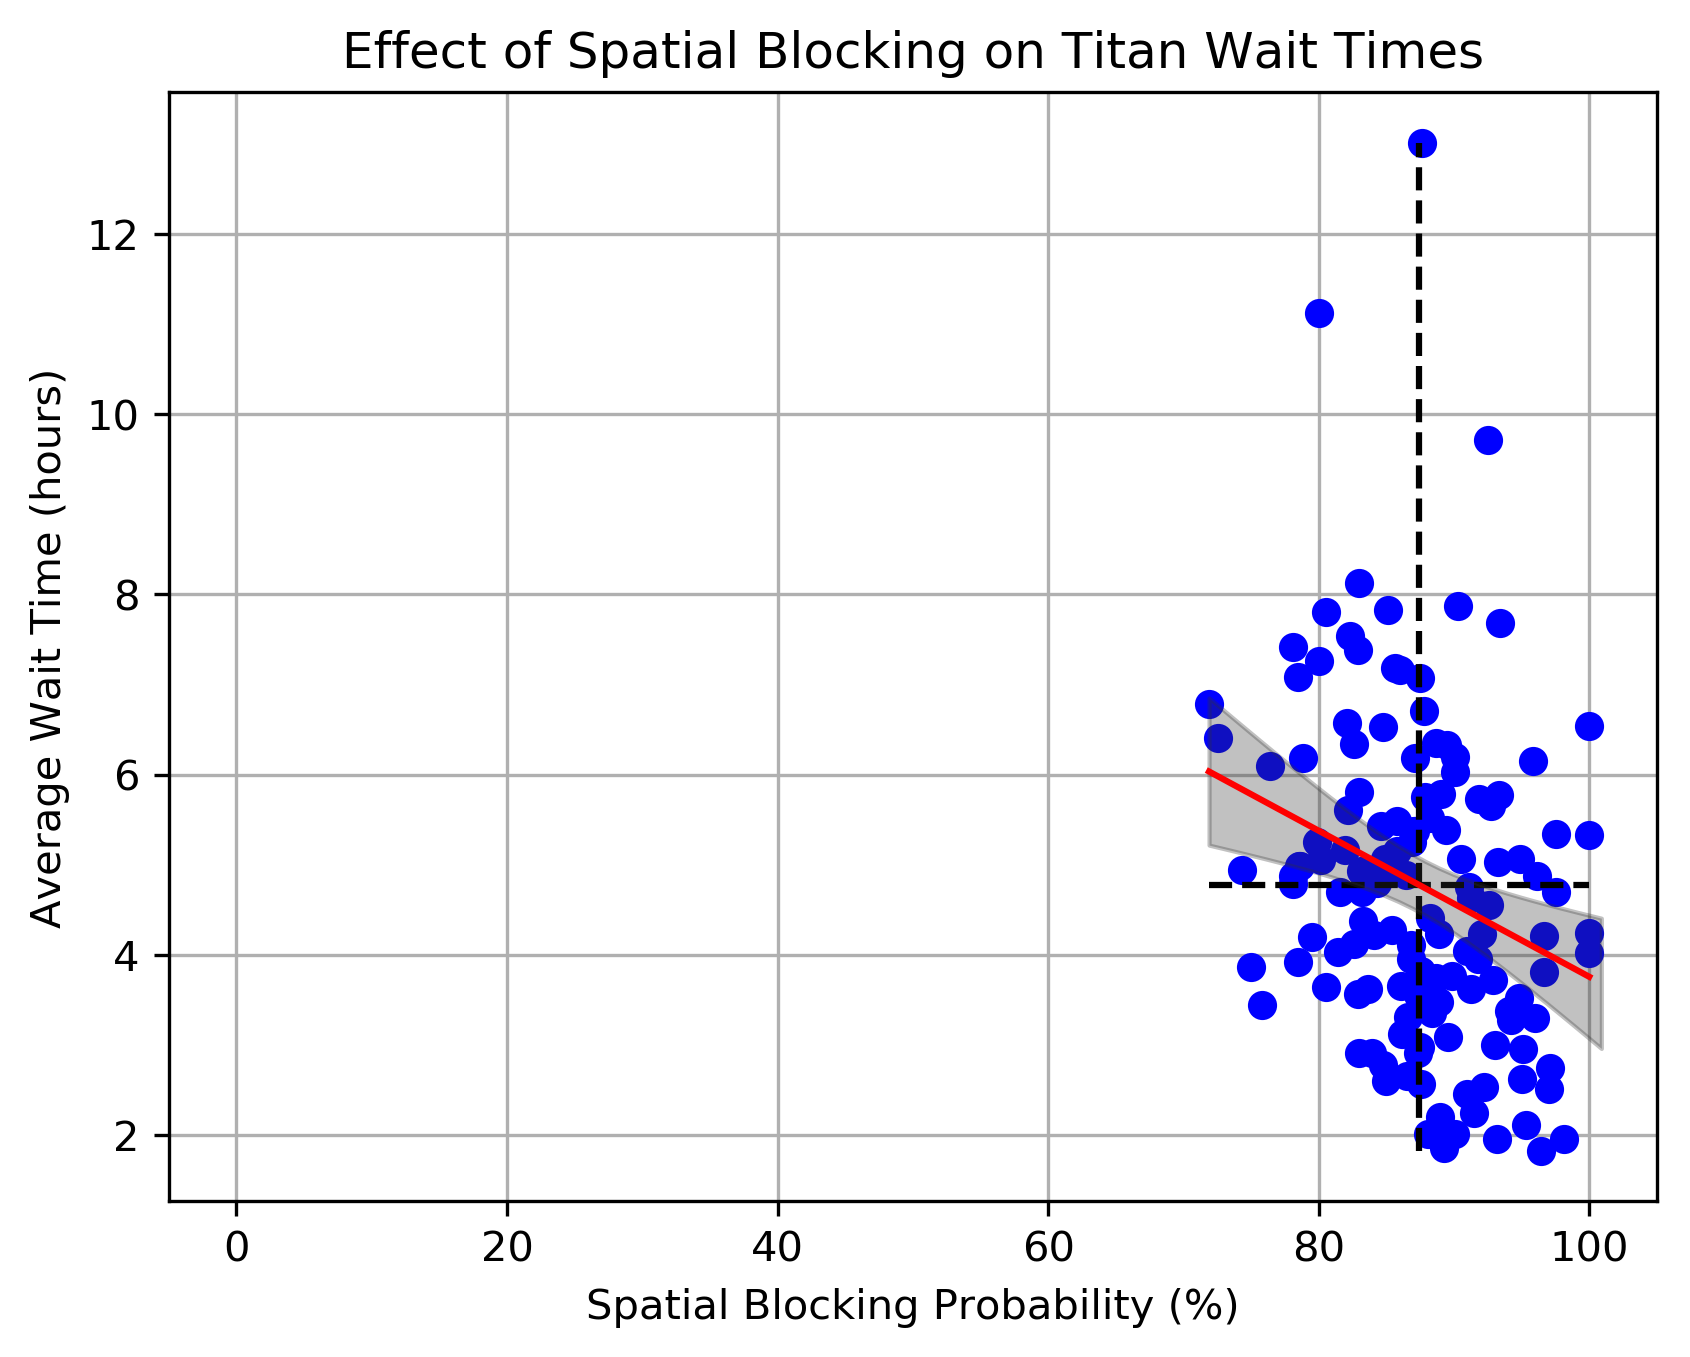
\includegraphics[width=0.4\textwidth]{images/linfit-wait-time-vs-spatial-blocking-by-day.png}}
  \subfloat[Temporal blocking\label{fig:wait-time-temporal-all}]{
    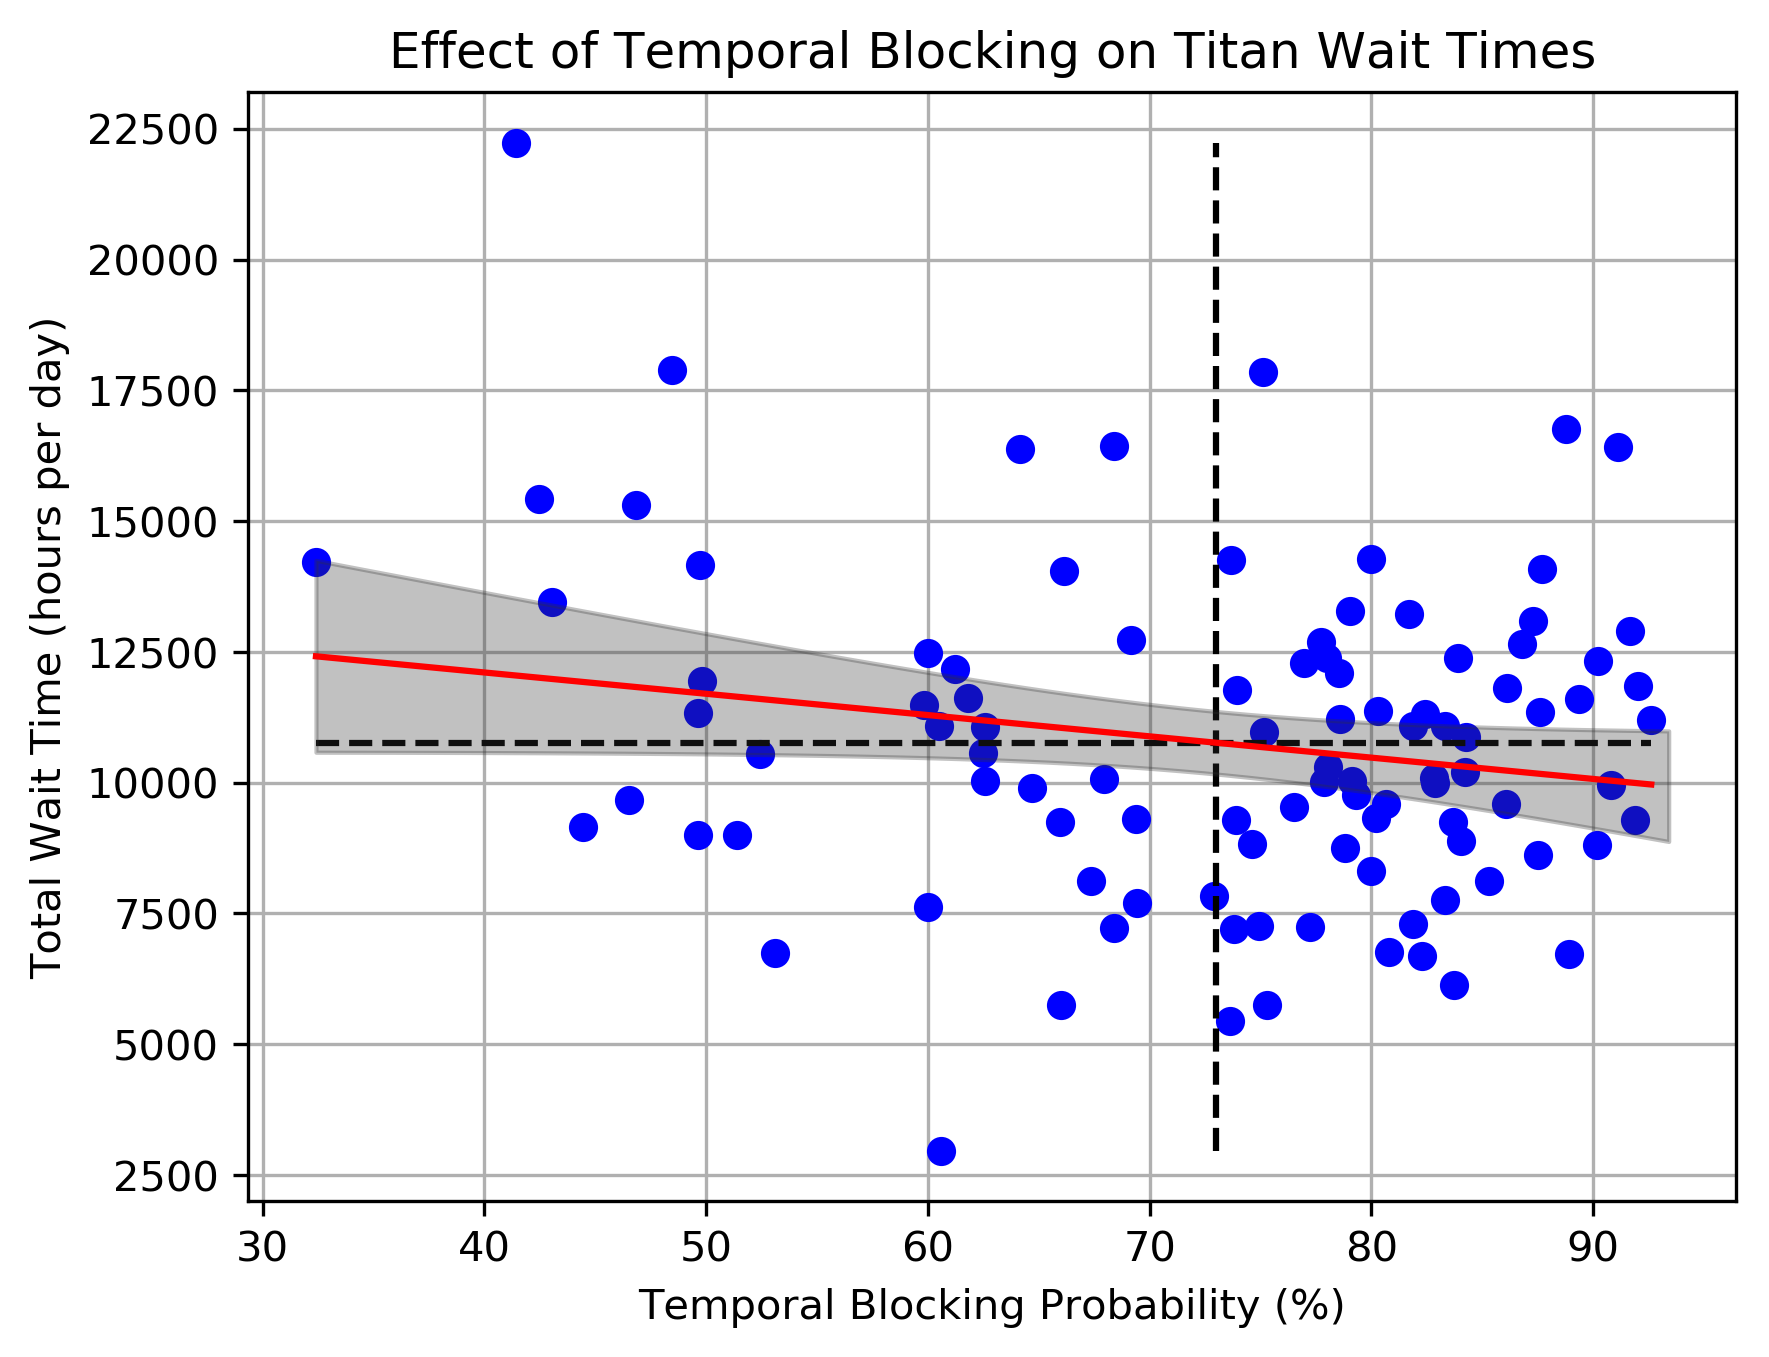
\includegraphics[width=0.4\textwidth]{images/linfit-wait-time-vs-temporal-blocking-by-day.png}}
  \vspace{1em}
  \subfloat[Spatial blocking by CSC108\label{fig:wait-time-spatial-csc108}]{
    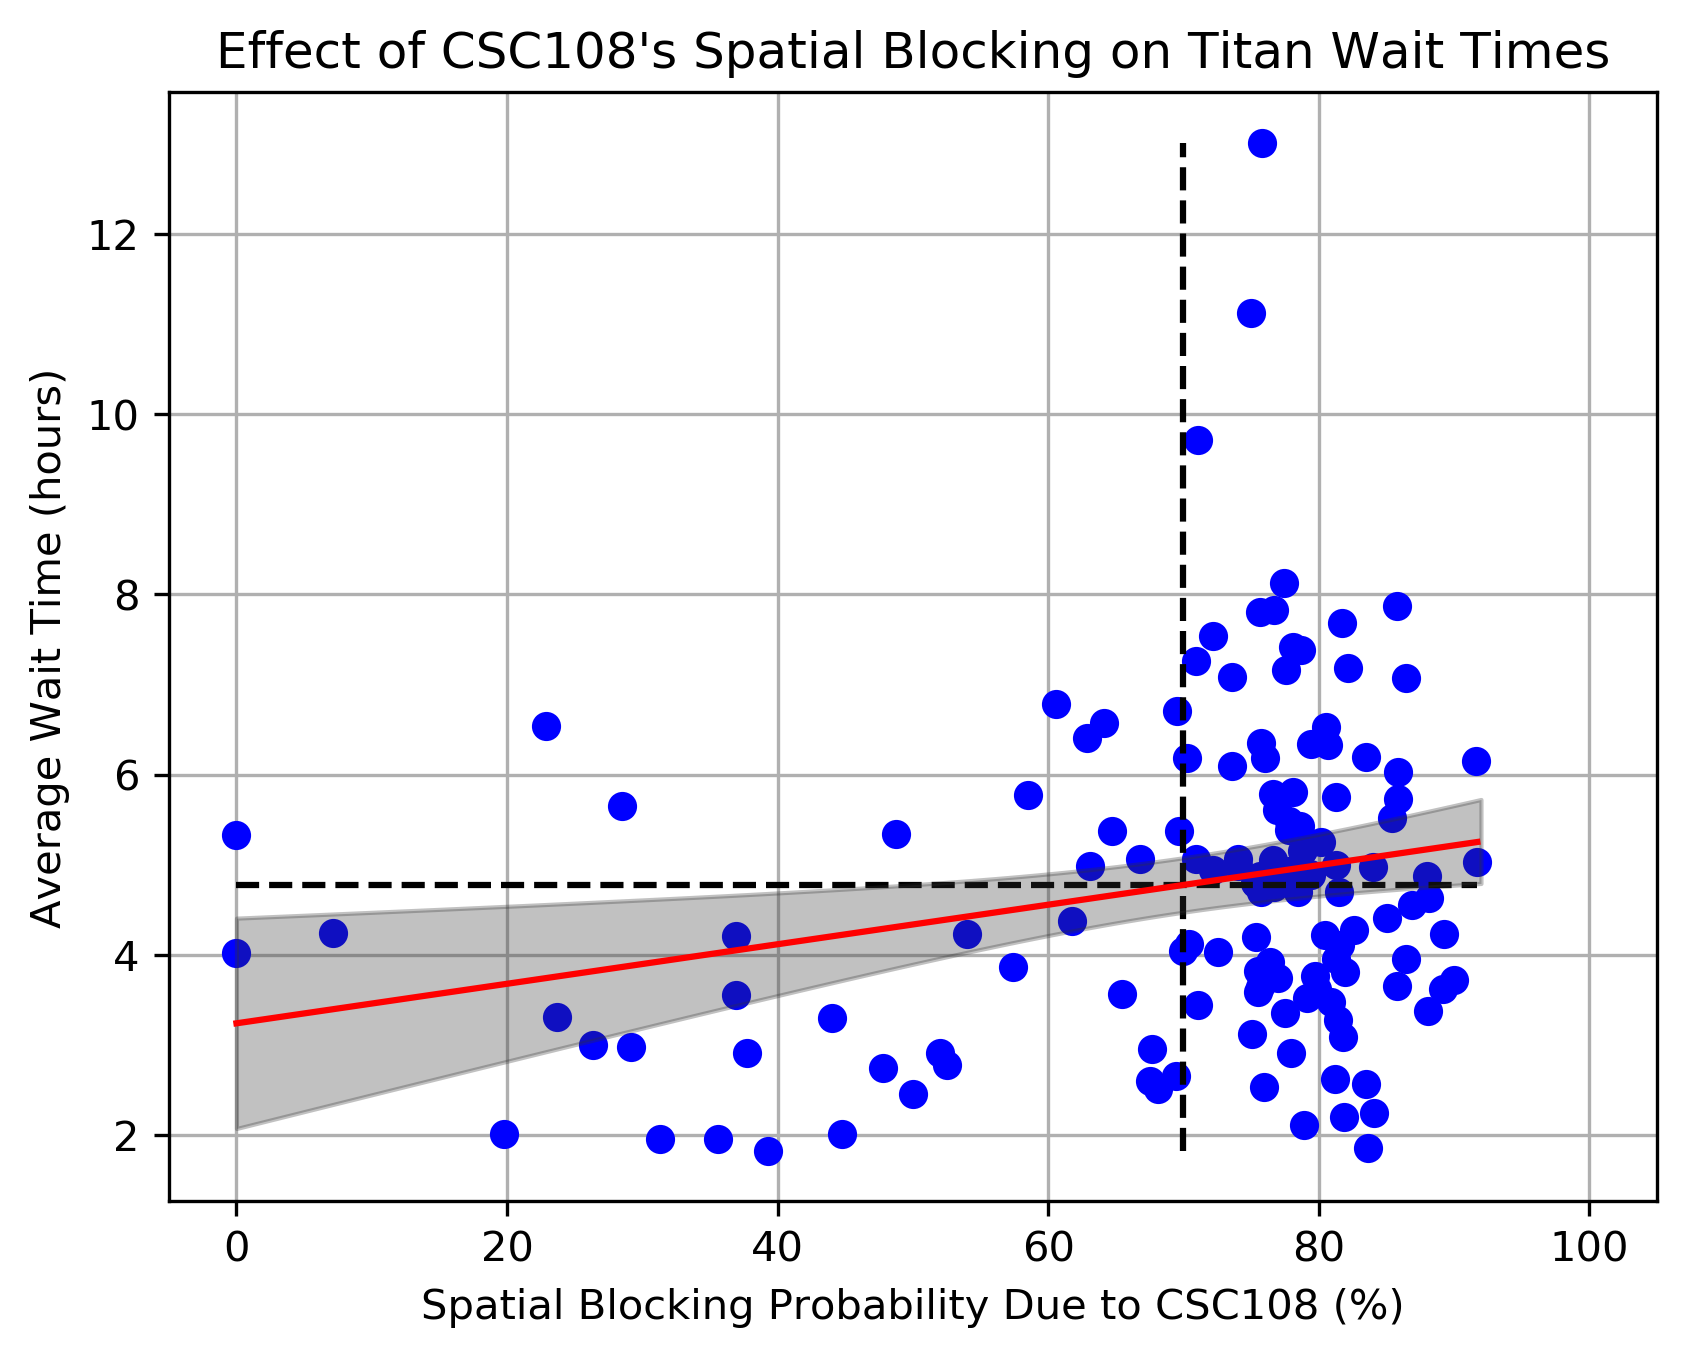
\includegraphics[width=0.4\textwidth]{images/linfit-wait-time-vs-csc108-spatial.png}}
  \subfloat[Temporal blocking by CSC108\label{fig:wait-time-temporal-csc108}]{
    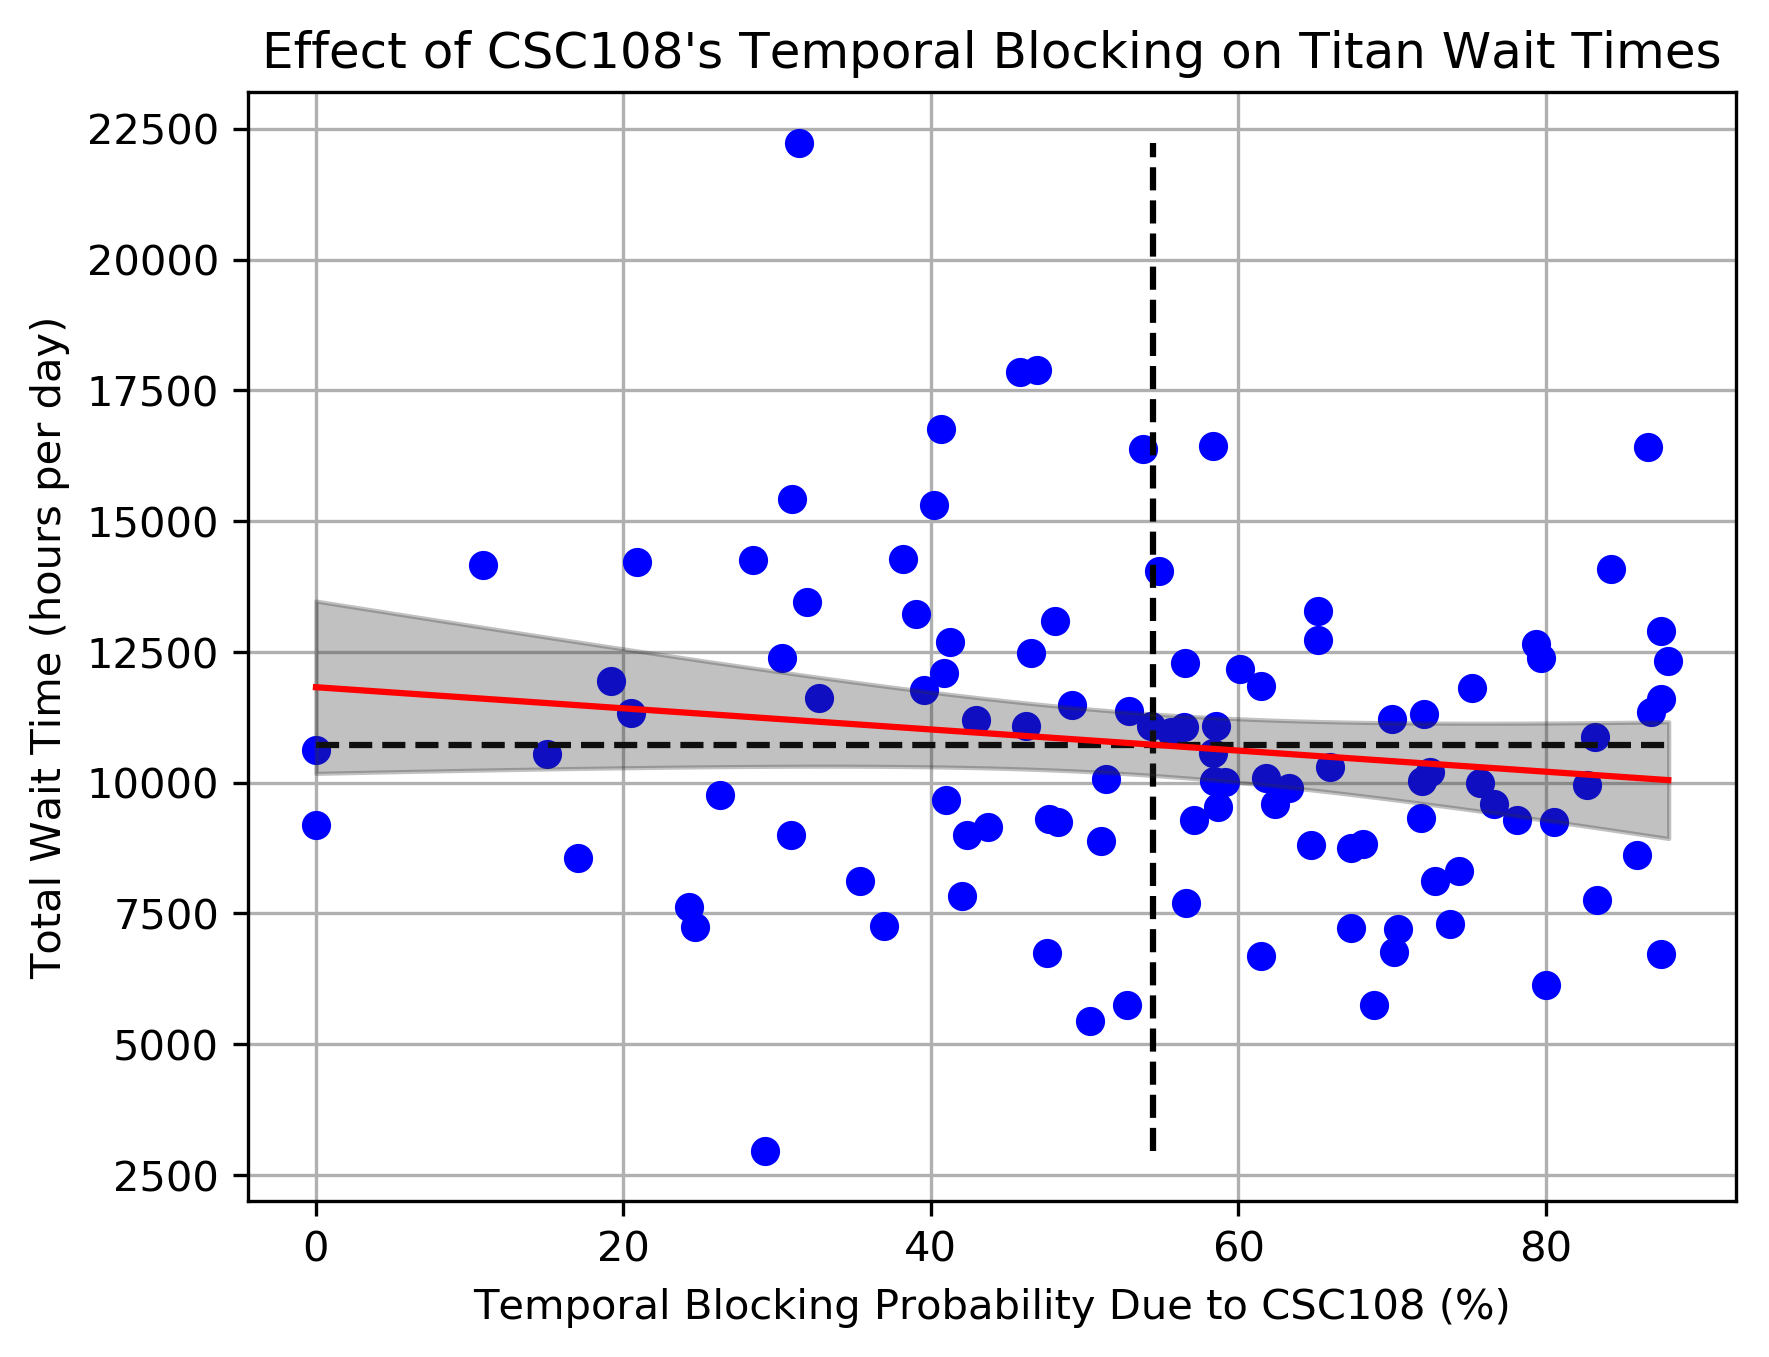
\includegraphics[width=0.4\textwidth]{images/linfit-wait-time-vs-csc108-temporal.png}}
  \caption{These plots demonstrate the relationships between the average wait
times on Titan and one-dimensional blocking probabilities. Each blue point
represents one day. Each red line is an Ordinary Least Squares (OLS) linear
regression with parameters given in Table~\ref{tab:blocking-wait-time-params}.
Each shaded gray area represents a 95\% confidence region. Each horizontal
dotted black line represents the mean wait times for all points in that plot,
and each vertical dotted black line represents the mean blocking probability
for all points in that plot.}
\end{figure*}

% For tables use
\begin{table}
% table caption is above the table
\caption{The table contains the parameter values for the Ordinary Least Squares
(OLS) linear regression models regarding blocking probabilities and average
wait times. The first column corresponds to the figure depicting the model,
while the second and third columns correspond the coefficients $\beta_1$ and
$\beta_0$ in the model $y = \beta_{1}x + \beta_0$.}
\label{tab:blocking-wait-time-params}       % Give a unique label
% For LaTeX tables use
\begin{tabular}{crrr}
\hline\noalign{\smallskip}
Figure  & Slope $\beta_1$ & Intercept $\beta_0$     & $\text{R}^2$ \\
\noalign{\smallskip}\hline\noalign{\smallskip}
\ref{fig:wait-time-spatial-all}     &   -0.0810 &   11.8610 &   0.0737  \\
\ref{fig:wait-time-temporal-all}    &   -0.0401 &    7.7491 &   0.1265  \\
\ref{fig:wait-time-spatial-csc108}  &    0.0219 &    3.2420 &   0.0509  \\
\ref{fig:wait-time-temporal-csc108} &   -0.0102 &    5.3217 &   0.0147  \\
\noalign{\smallskip}\hline
\end{tabular}
\end{table}

%%% THROUGHPUT STUFF

Figures \ref{fig:throughput-spatial-all}, \ref{fig:throughput-temporal-all},
\ref{fig:throughput-spatial-csc108}, and \ref{fig:throughput-temporal-csc108}
are all in agreement that increasing competition corresponds to increasing
throughput, in units of jobs completed per day. The goodness-of-fit values are
poor, however, as shown in Table~\ref{tab:blocking-throughput-params}, so these qualitative results may only be said to be suggestive.

%%%
\begin{figure*}
  \subfloat[Spatial blocking\label{fig:throughput-spatial-all}]{
    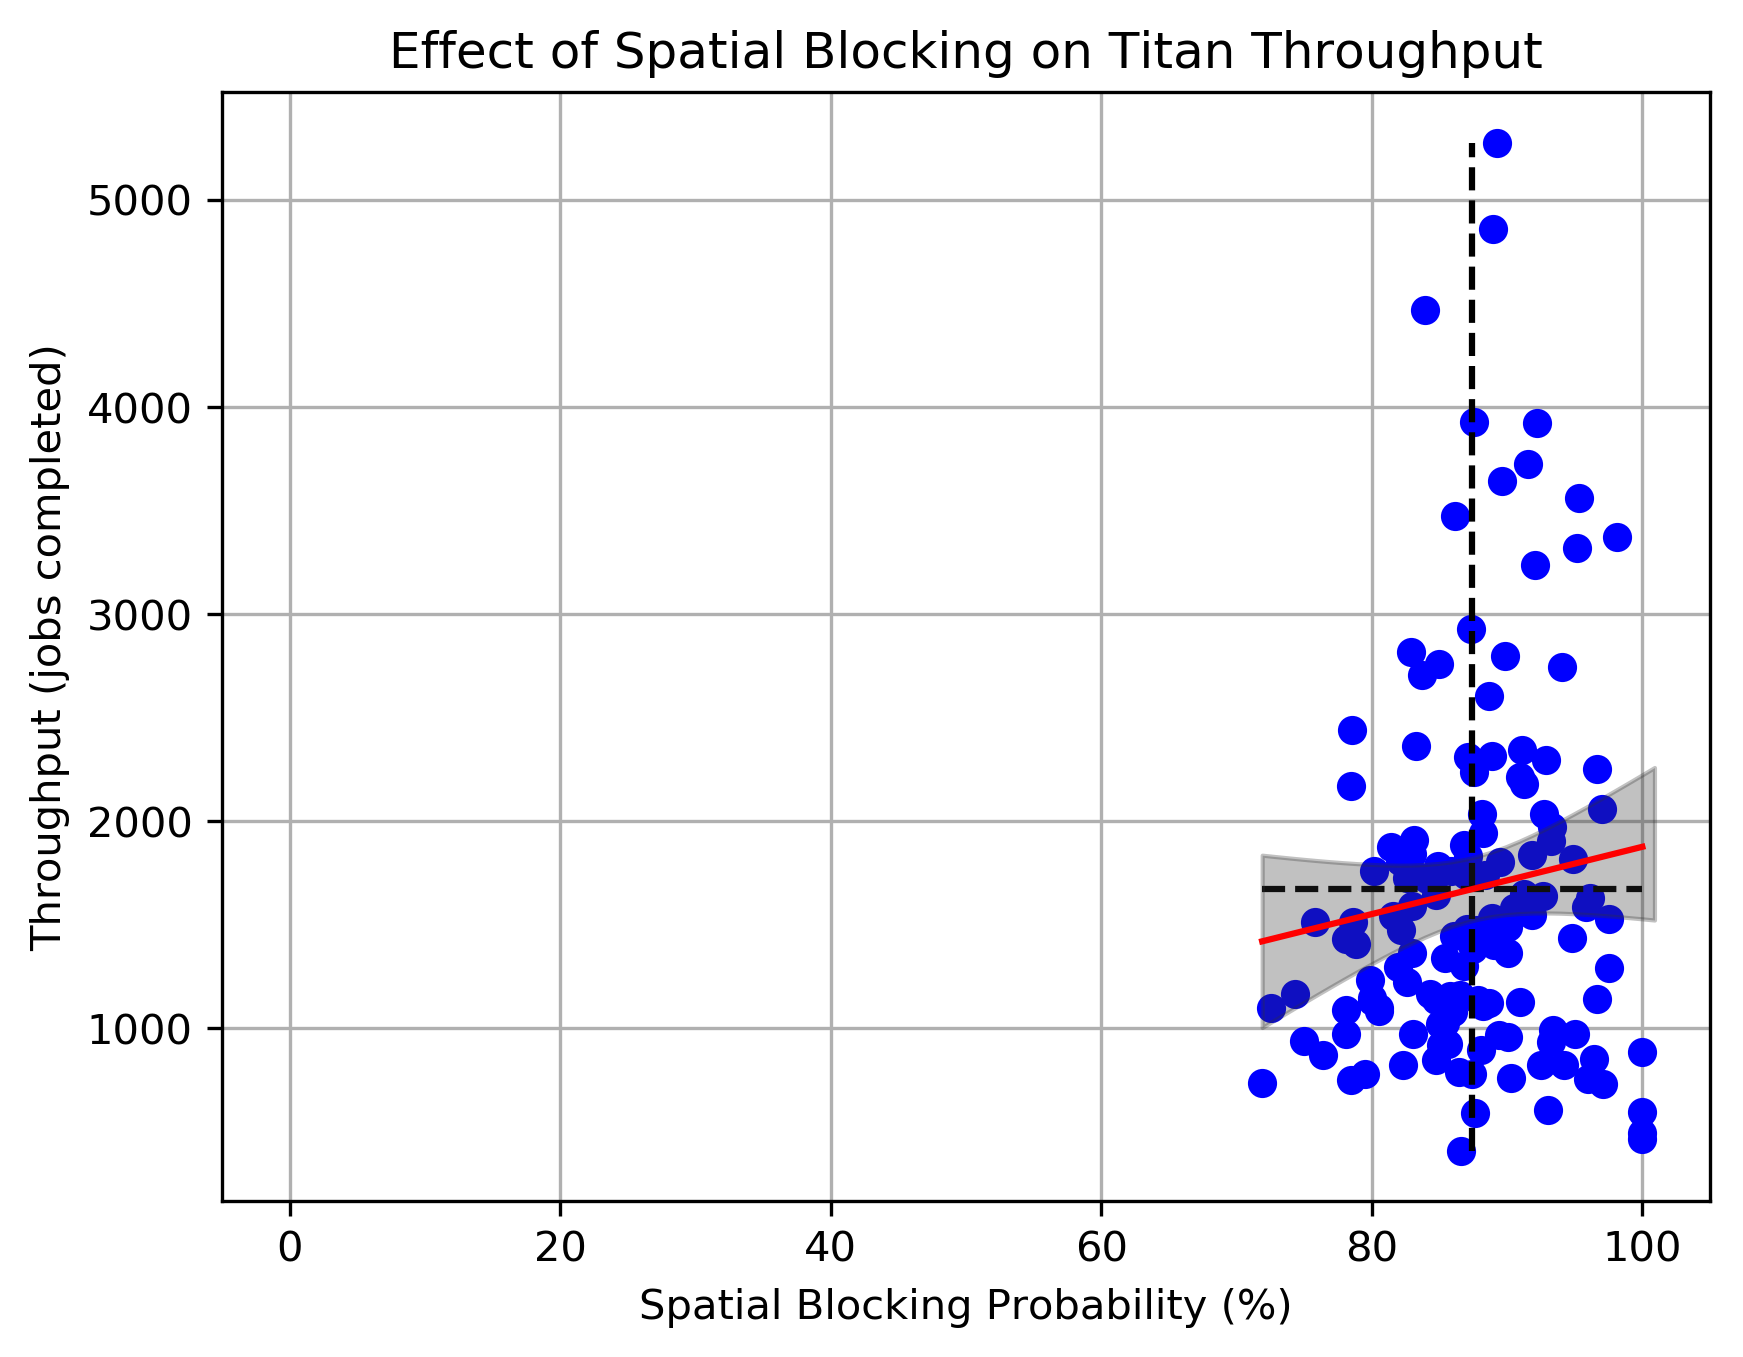
\includegraphics[width=0.4\textwidth]{images/linfit-throughput-vs-spatial-blocking.png}}
  \subfloat[Temporal blocking\label{fig:throughput-temporal-all}]{
    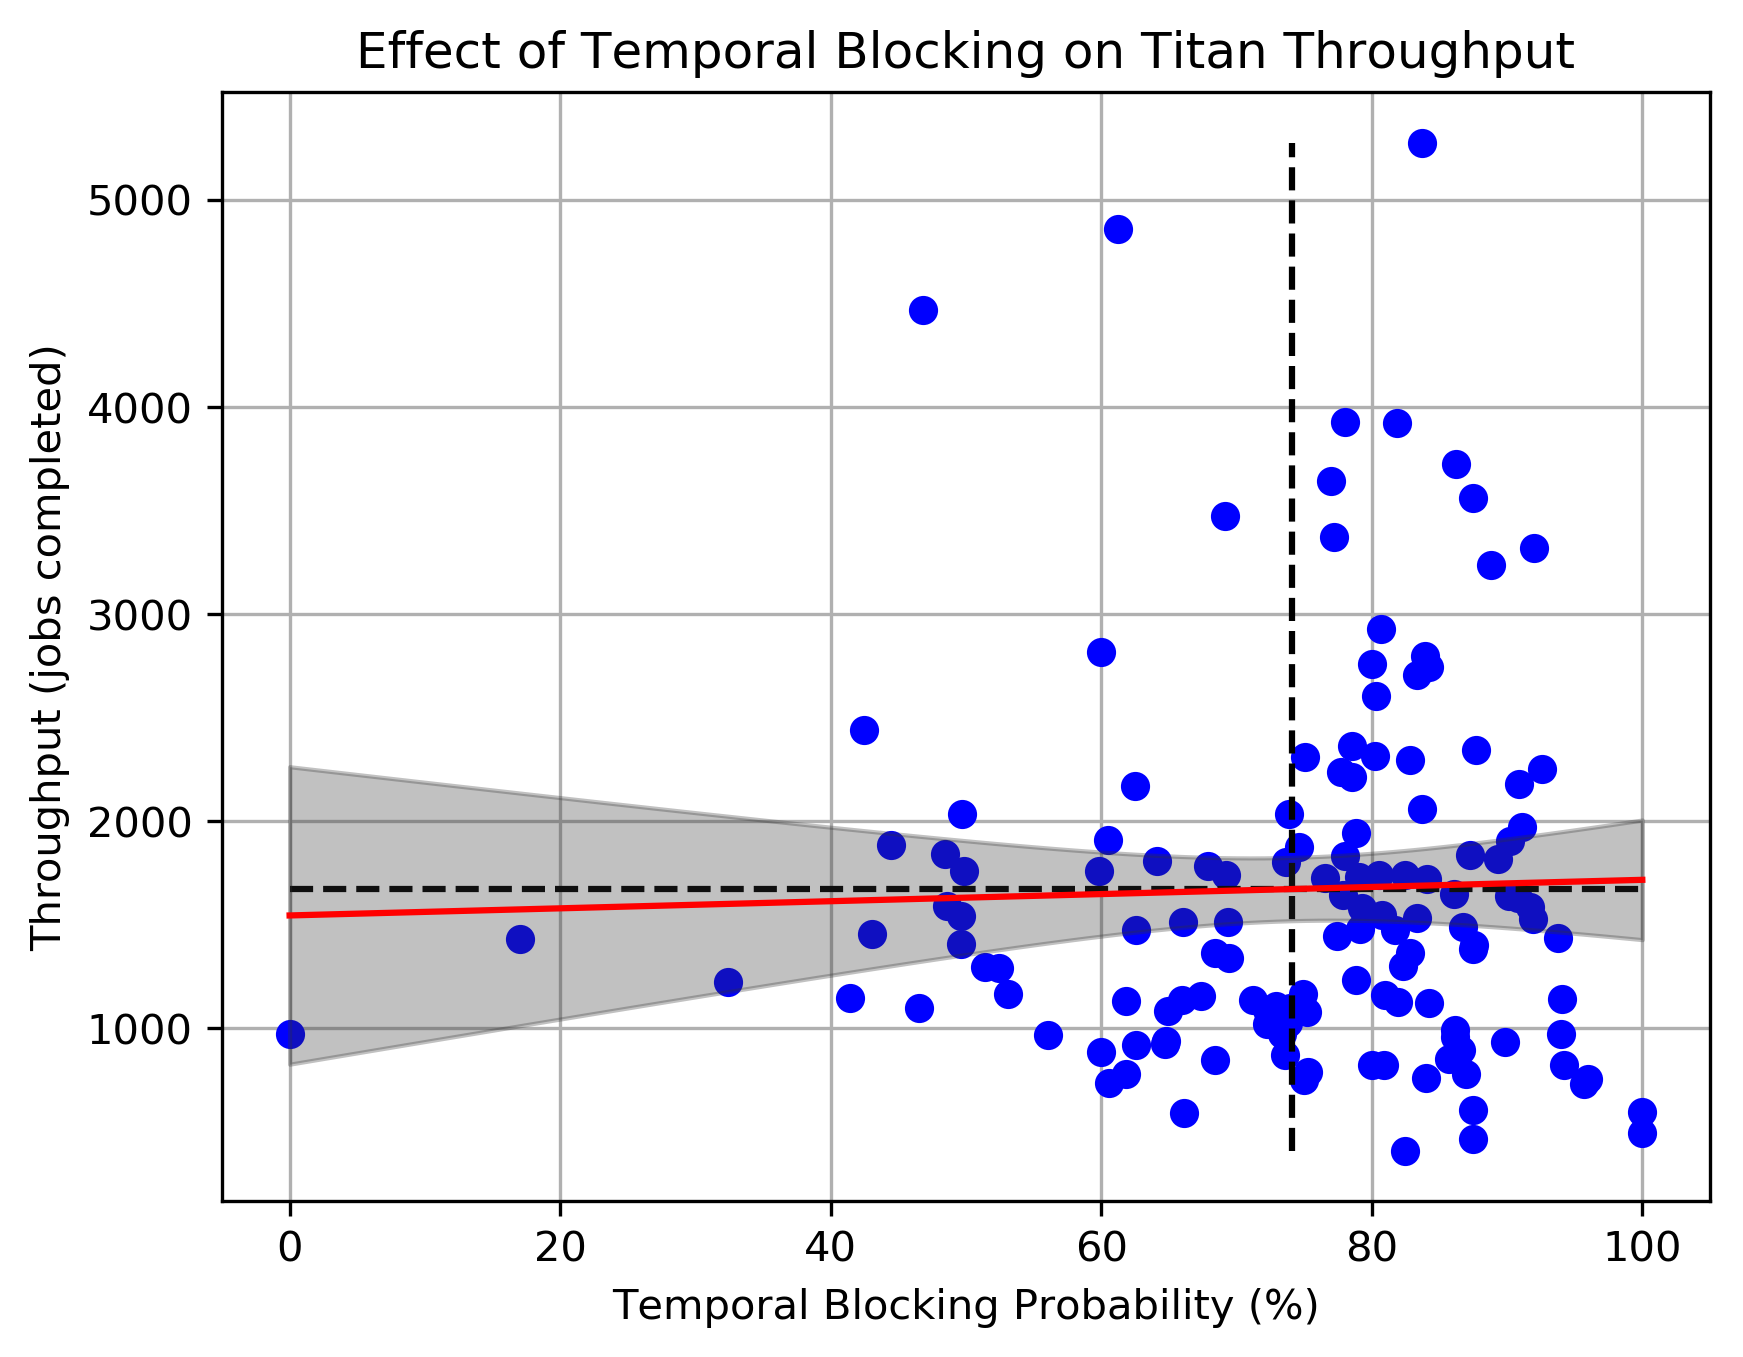
\includegraphics[width=0.4\textwidth]{images/linfit-throughput-vs-temporal-blocking.png}}
  \vspace{1em}
  \subfloat[Spatial blocking by CSC108\label{fig:throughput-spatial-csc108}]{
    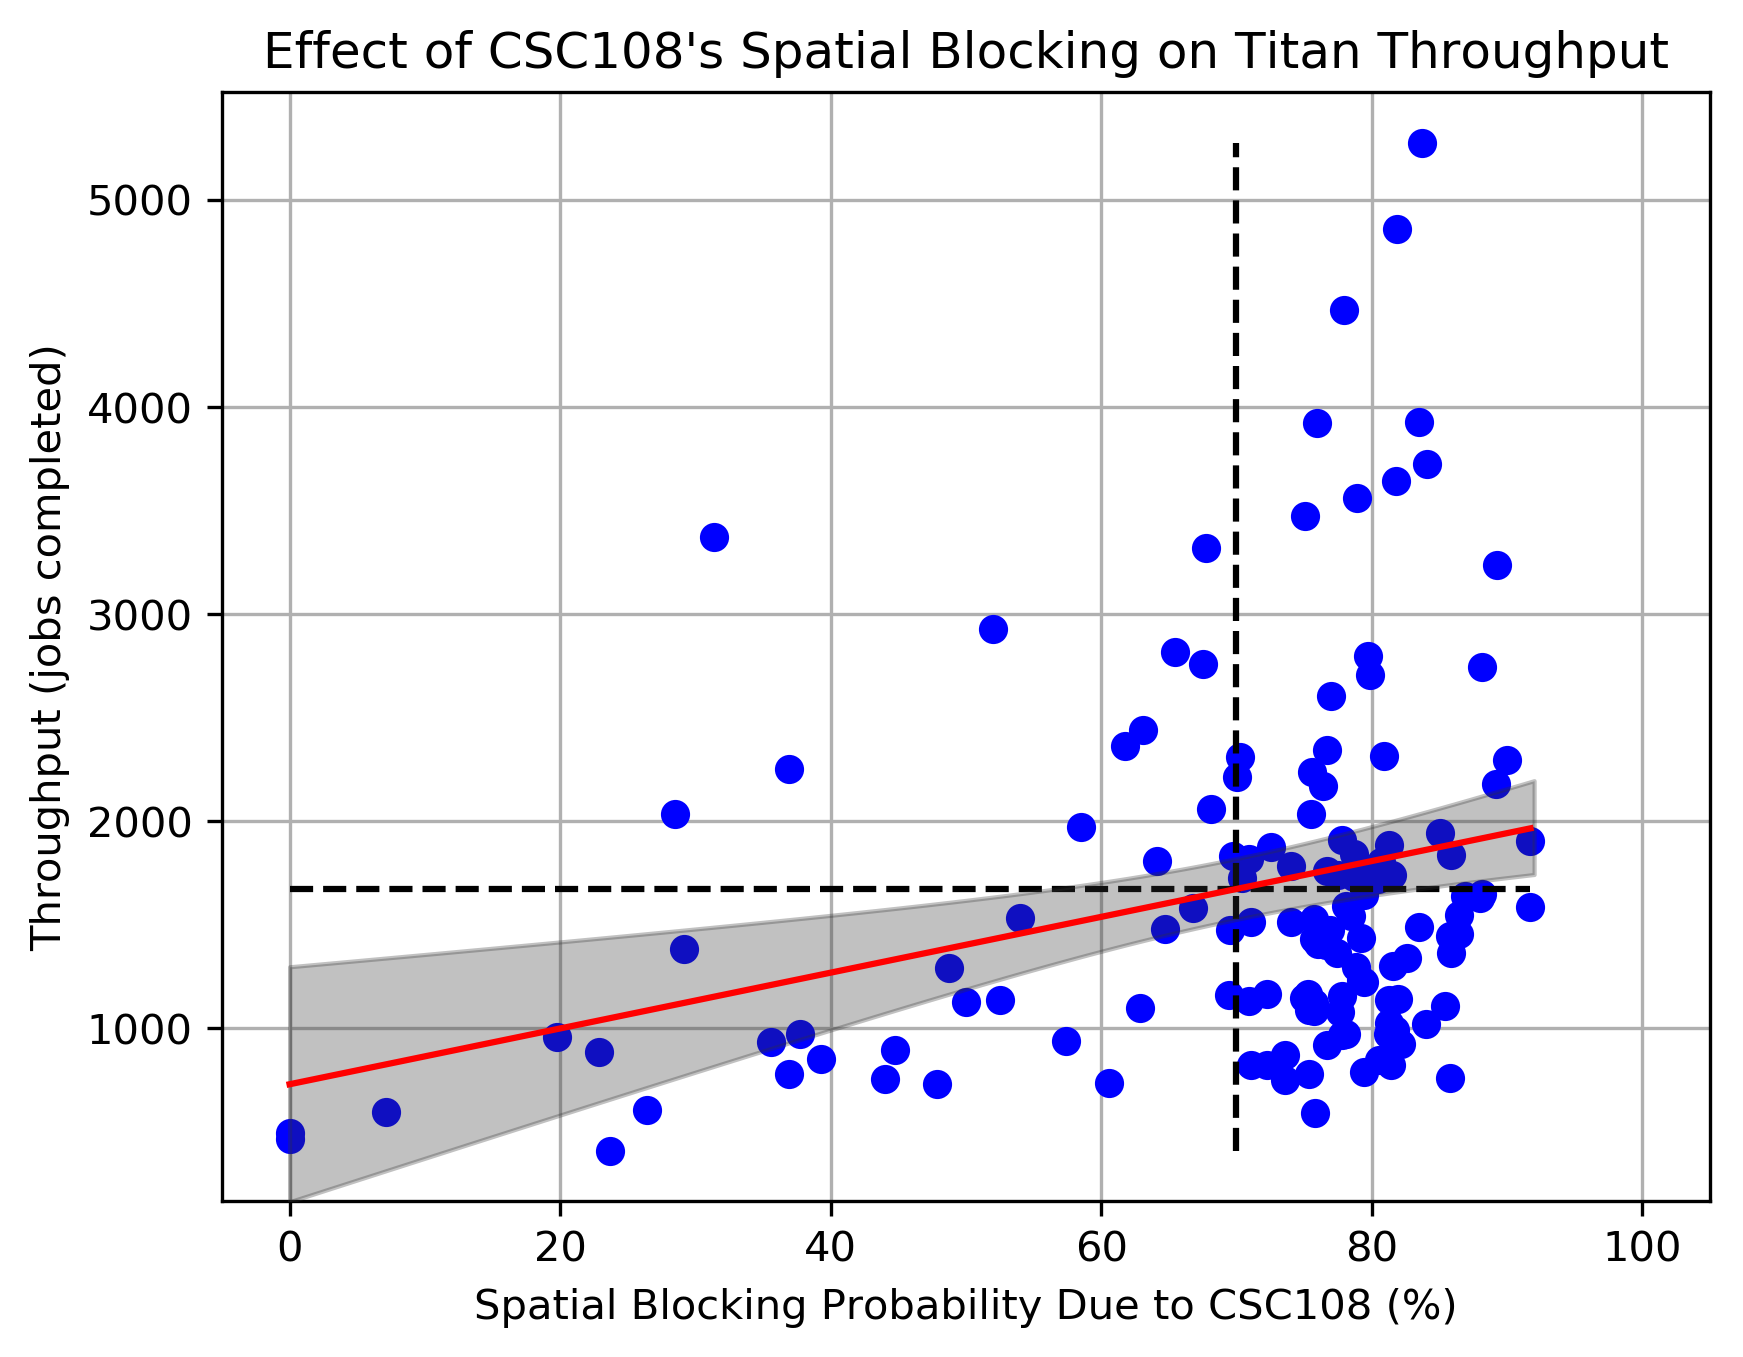
\includegraphics[width=0.4\textwidth]{images/linfit-throughput-vs-csc108-spatial.png}}
  \subfloat[Temporal blocking by CSC108\label{fig:throughput-temporal-csc108}]{
    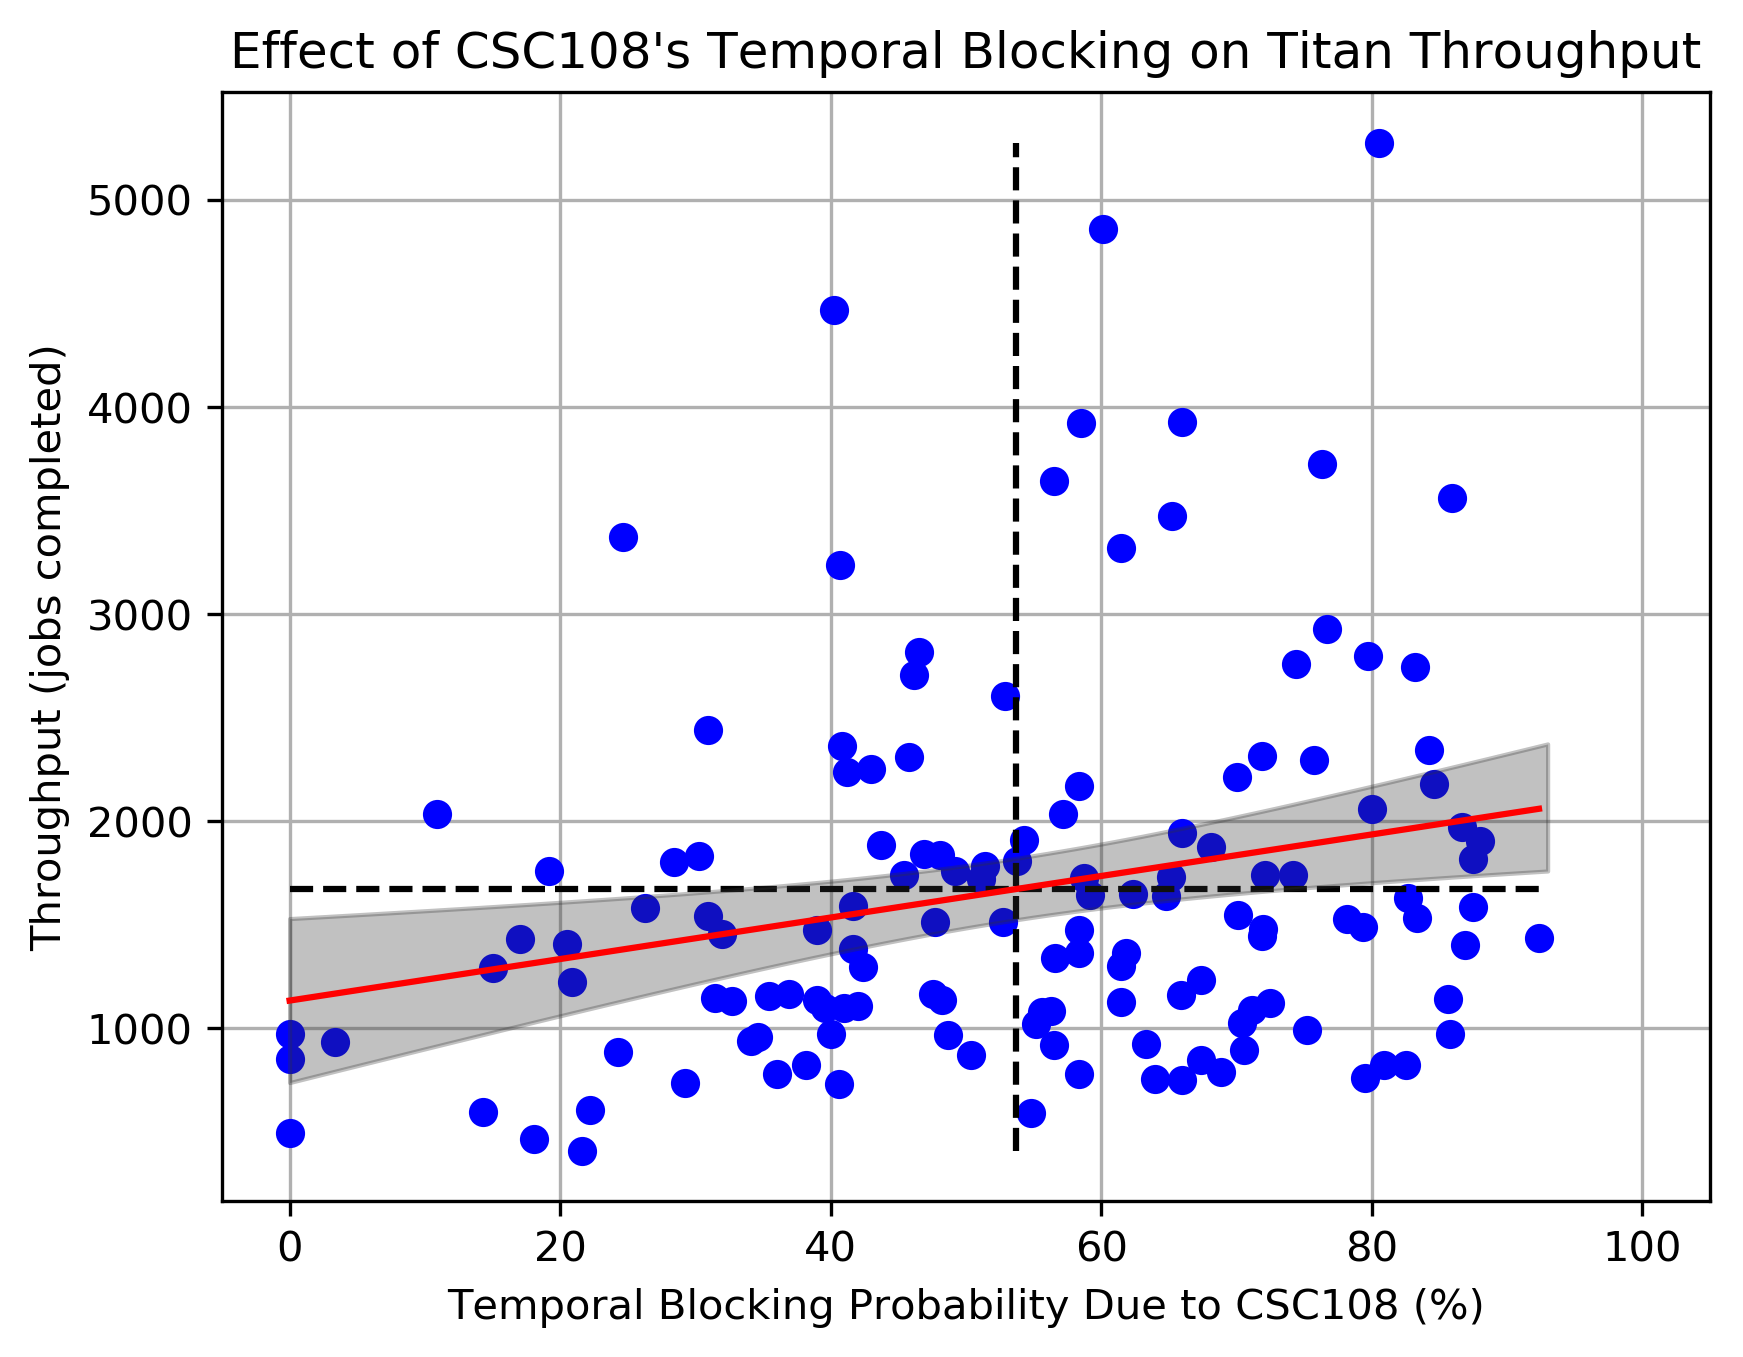
\includegraphics[width=0.4\textwidth]{images/linfit-throughput-vs-csc108-temporal.png}}
  \caption{These plots demonstrate the relationships between throughput on
Titan and one-dimensional blocking probabilities. Each blue point represents
one day. Each red line is an Ordinary Least Squares (OLS) linear regression
with parameters given in Table~\ref{tab:blocking-throughput-params}. Each
shaded gray area represents a 95\% confidence region. Each horizontal dotted
black line represents the mean wait times for all points in that plot, and each
vertical dotted black line represents the mean blocking probability for all
points in that plot.}
\end{figure*}

% For tables use
\begin{table}
% table caption is above the table
\caption{The table contains the parameter values for the Ordinary Least Squares
(OLS) linear regression models regarding blocking probabilities and throughput.
The first column corresponds to the figure depicting the model, while the
second and third columns correspond the coefficients $\beta_1$ and $\beta_0$ in
the model $y = \beta_{1}x + \beta_0$.}
\label{tab:blocking-throughput-params}       % Give a unique label
% For LaTeX tables use
\begin{tabular}{crrr}
\hline\noalign{\smallskip}
Figure  & Slope $\beta_1$ & Intercept $\beta_0$     & $\text{R}^2$ \\
\noalign{\smallskip}\hline\noalign{\smallskip}
\ref{fig:throughput-spatial-all}     &  16.2402 &   252.3652    &   0.0122  \\
\ref{fig:throughput-temporal-all}    &   1.7196 &  1544.9669    &   0.0010  \\
\ref{fig:throughput-spatial-csc108}  &  13.4683 &   730.0687    &   0.0790  \\
\ref{fig:throughput-temporal-csc108} &  10.0245 &  1134.0212    &   0.0587  \\
\noalign{\smallskip}\hline
\end{tabular}
\end{table}
%%%

%%% UTILIZATION STUFF

Finally, we searched for simple linear relationships between the different
blocking probabilities and overall utilization on Titan. Figures
\ref{fig:utilization-spatial-all}, \ref{fig:utilization-temporal-all},
\ref{fig:utilization-spatial-csc108}, and \ref{fig:utilization-temporal-csc108}
do not ``agree'' like the throughput plots did, but three plots suggest an
interpretation in which increasing competition, indicated by increasing
blocking probability, corresponds to decreased utilization. The fourth plot,
which indicates competition with CSC108, relates increased competition to
increased utilization. Once again, the goodness-of-fit values are poor, as
shown in Table~\ref{tab:blocking-utilization-params}.

%%%
\begin{figure*}
  \subfloat[Spatial blocking\label{fig:utilization-spatial-all}]{
    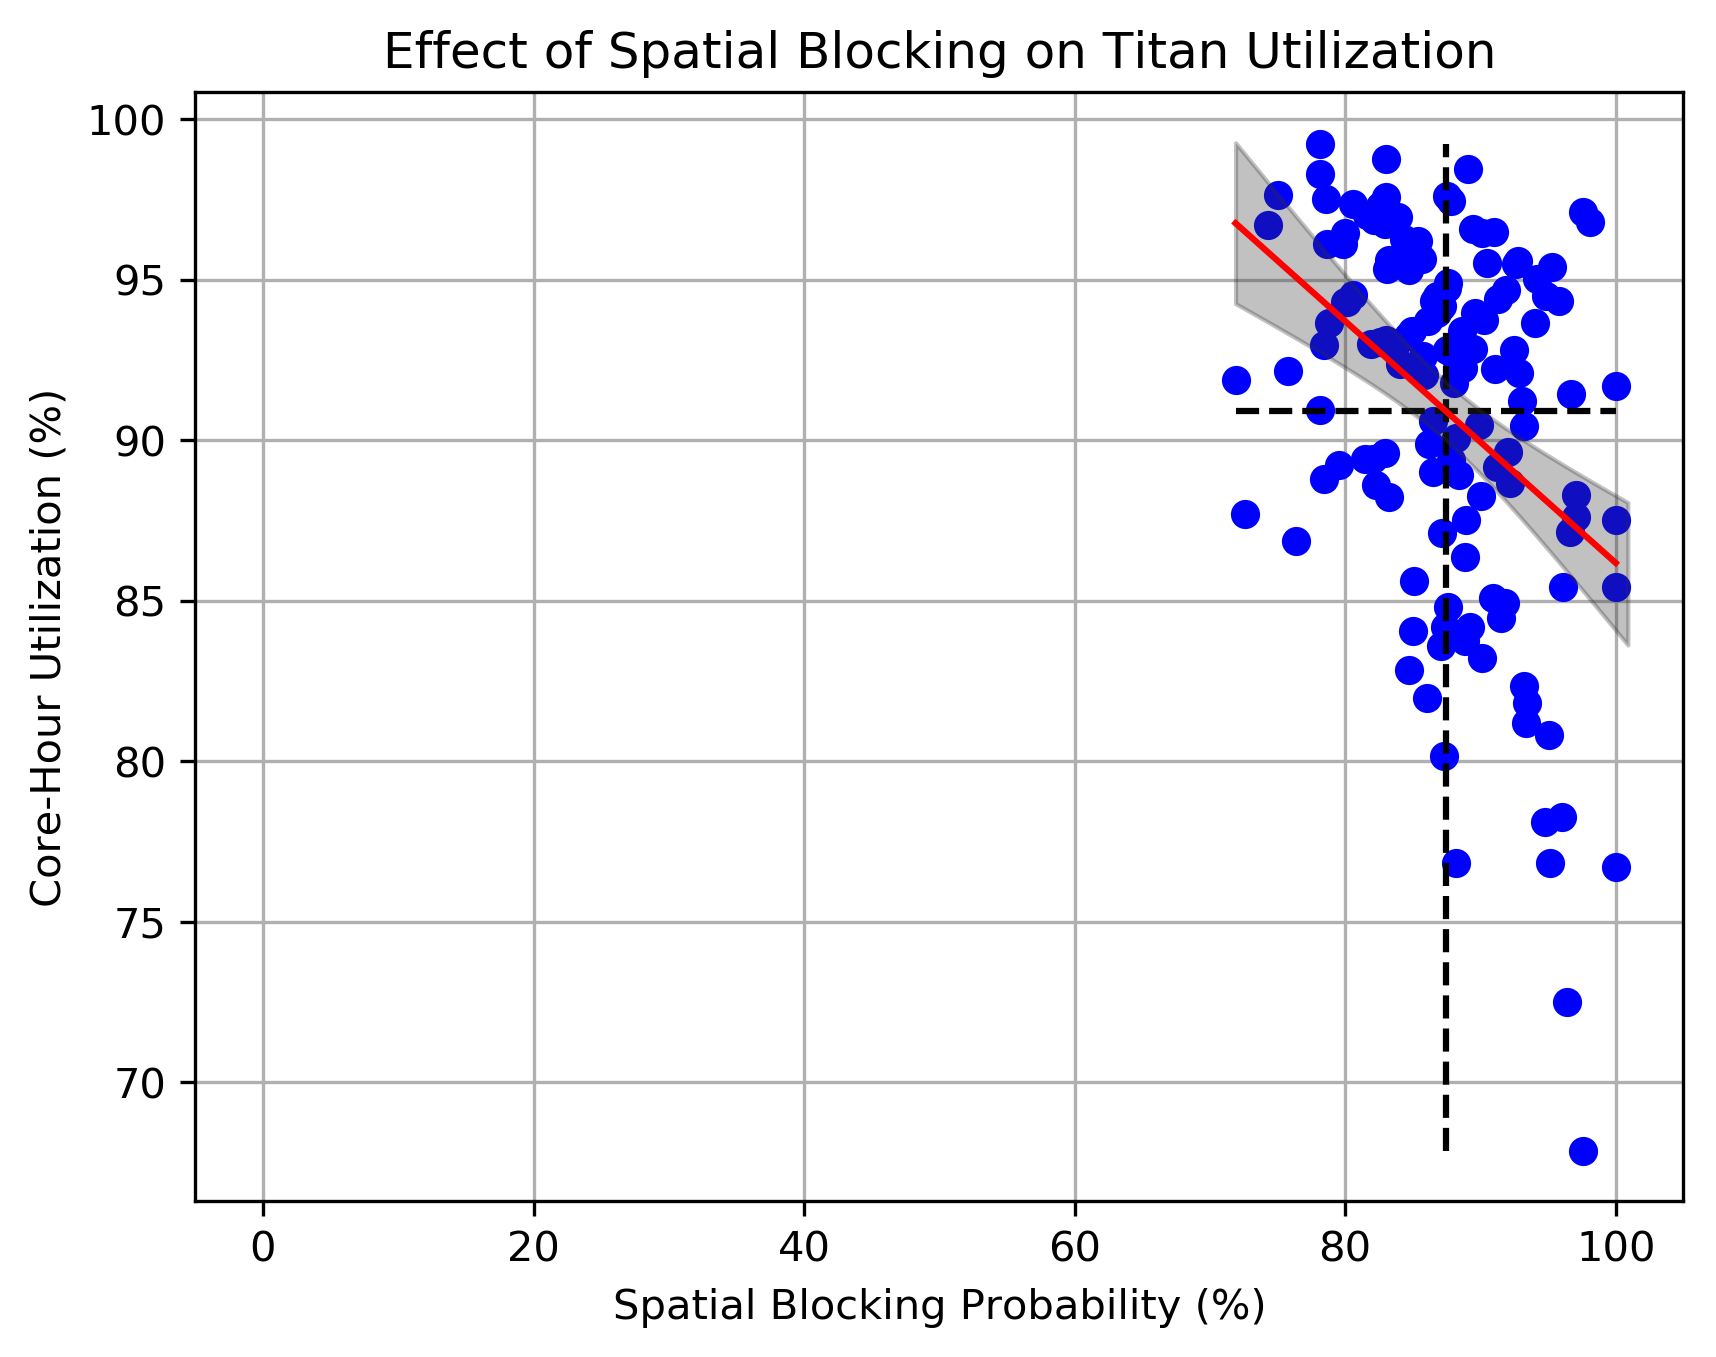
\includegraphics[width=0.4\textwidth]{images/linfit-utilization-vs-spatial-blocking.png}}
  \subfloat[Temporal blocking\label{fig:utilization-temporal-all}]{
    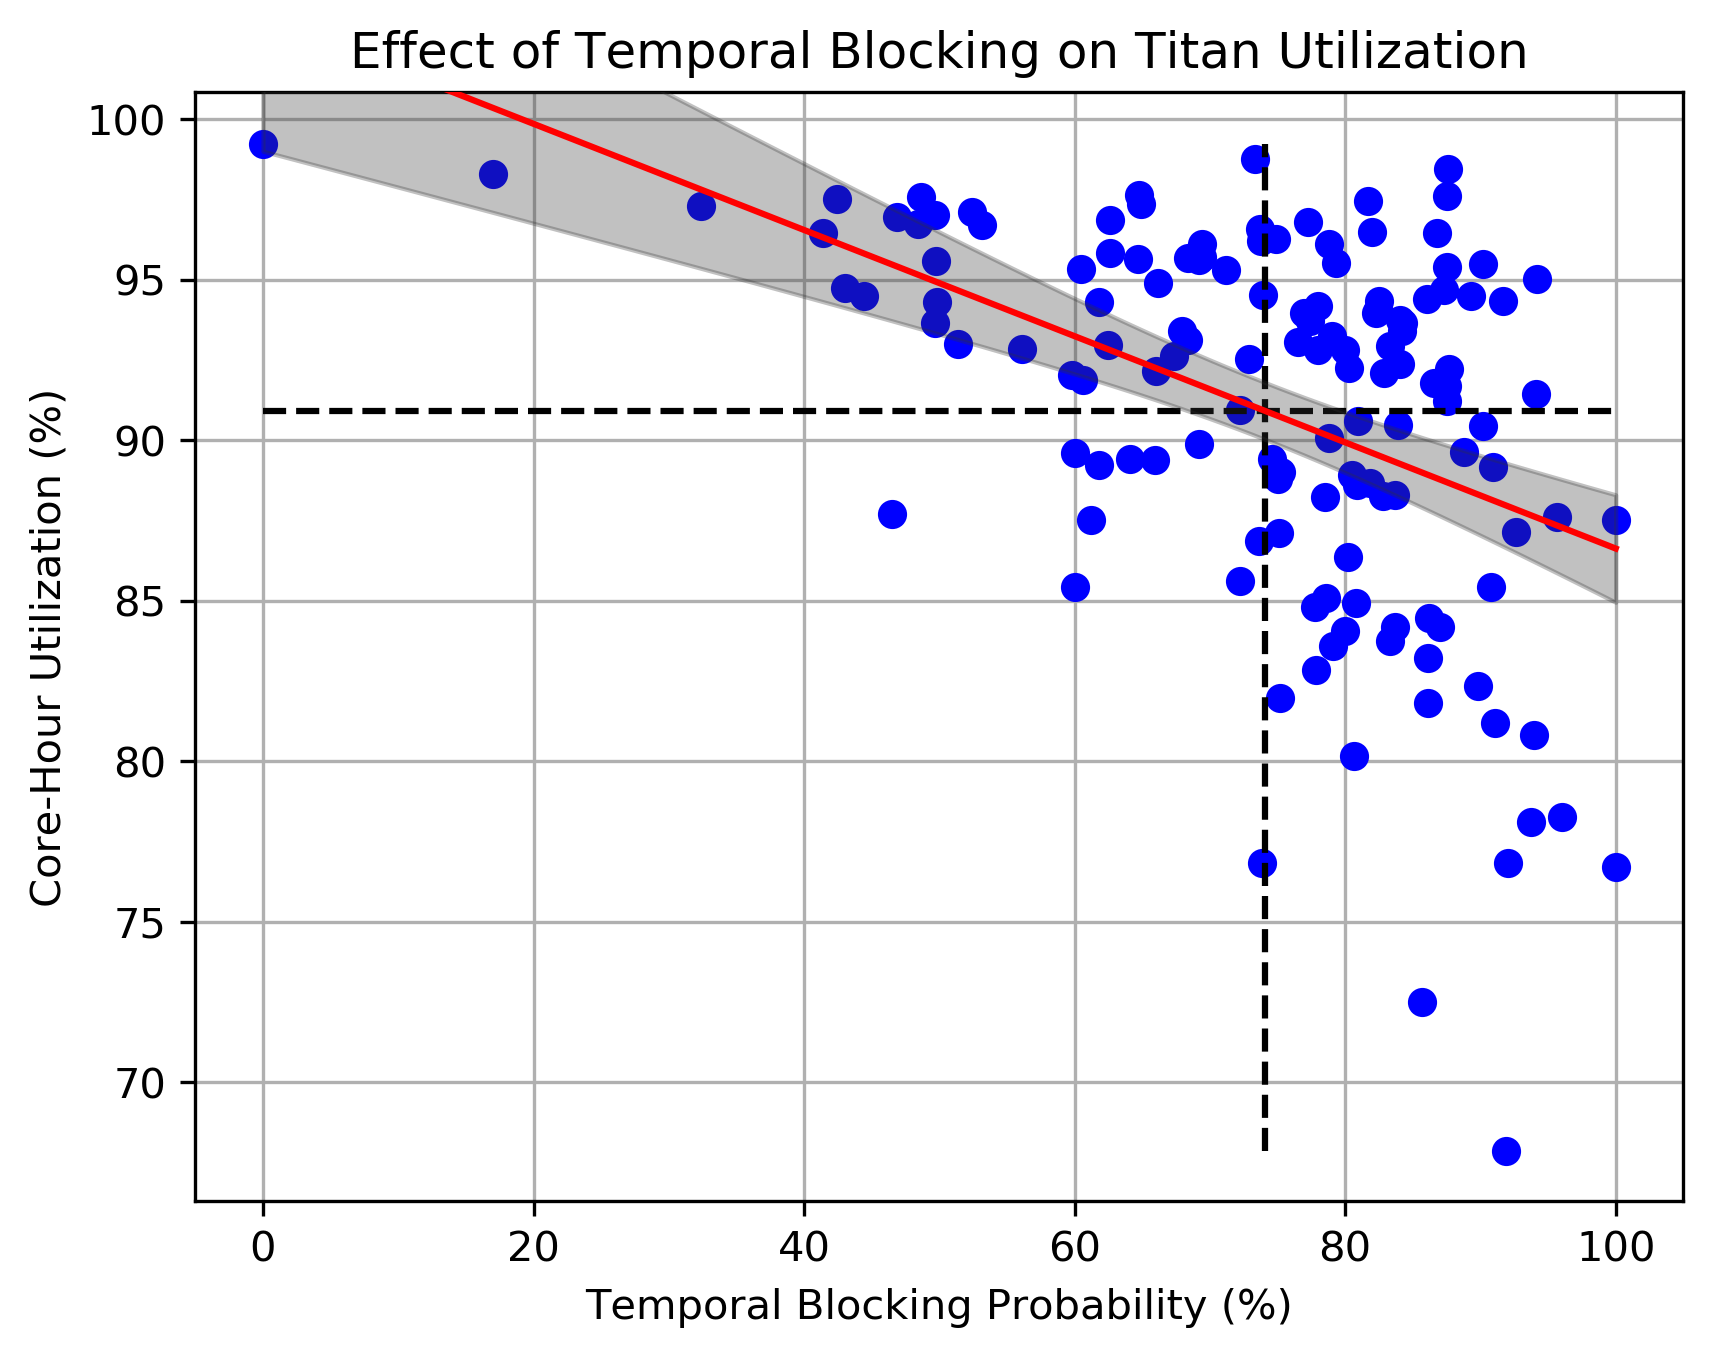
\includegraphics[width=0.4\textwidth]{images/linfit-utilization-vs-temporal-blocking.png}}
  \vspace{1em}
  \subfloat[Spatial blocking by CSC108\label{fig:utilization-spatial-csc108}]{
    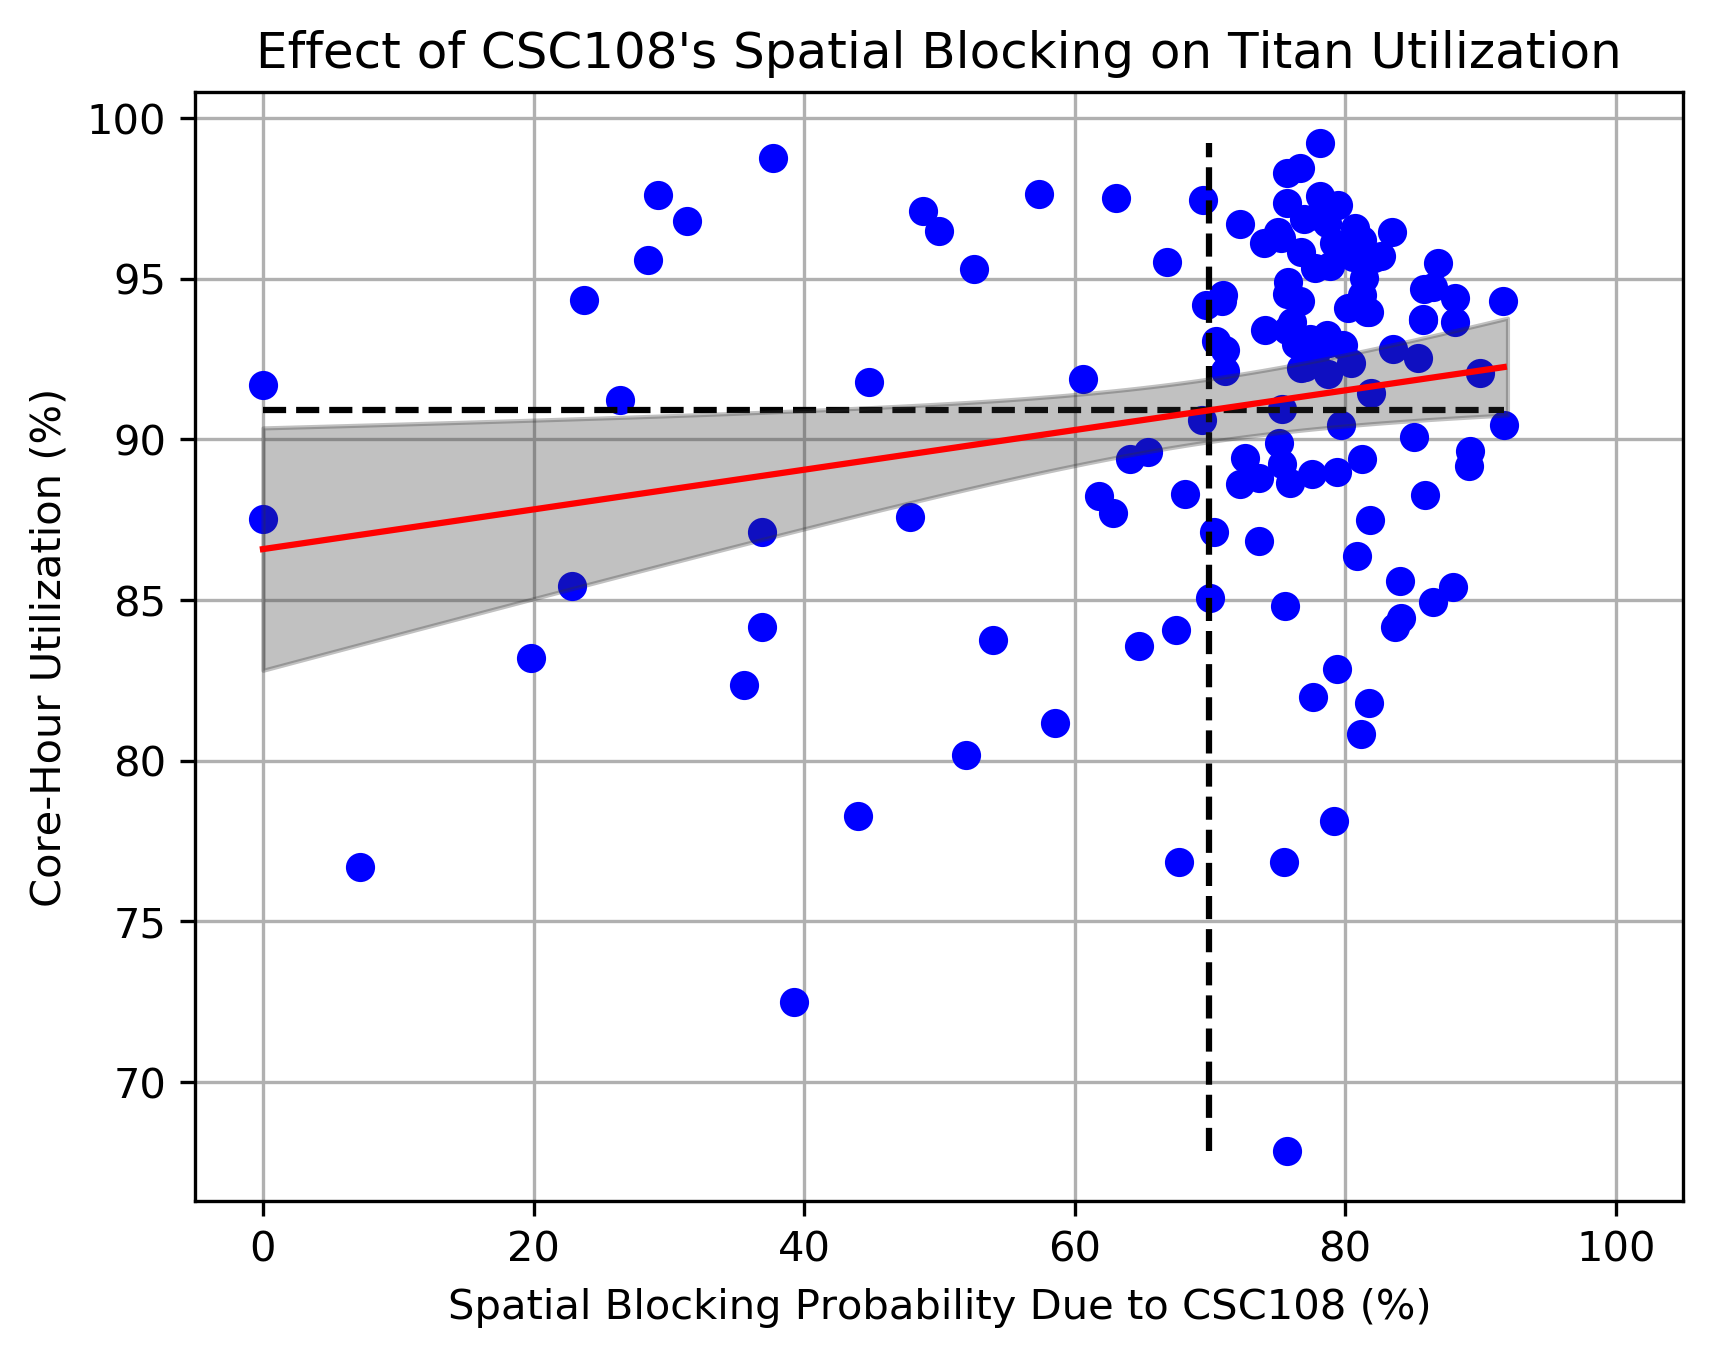
\includegraphics[width=0.4\textwidth]{images/linfit-utilization-vs-csc108-spatial.png}}
  \subfloat[Temporal blocking by CSC108\label{fig:utilization-temporal-csc108}]{
    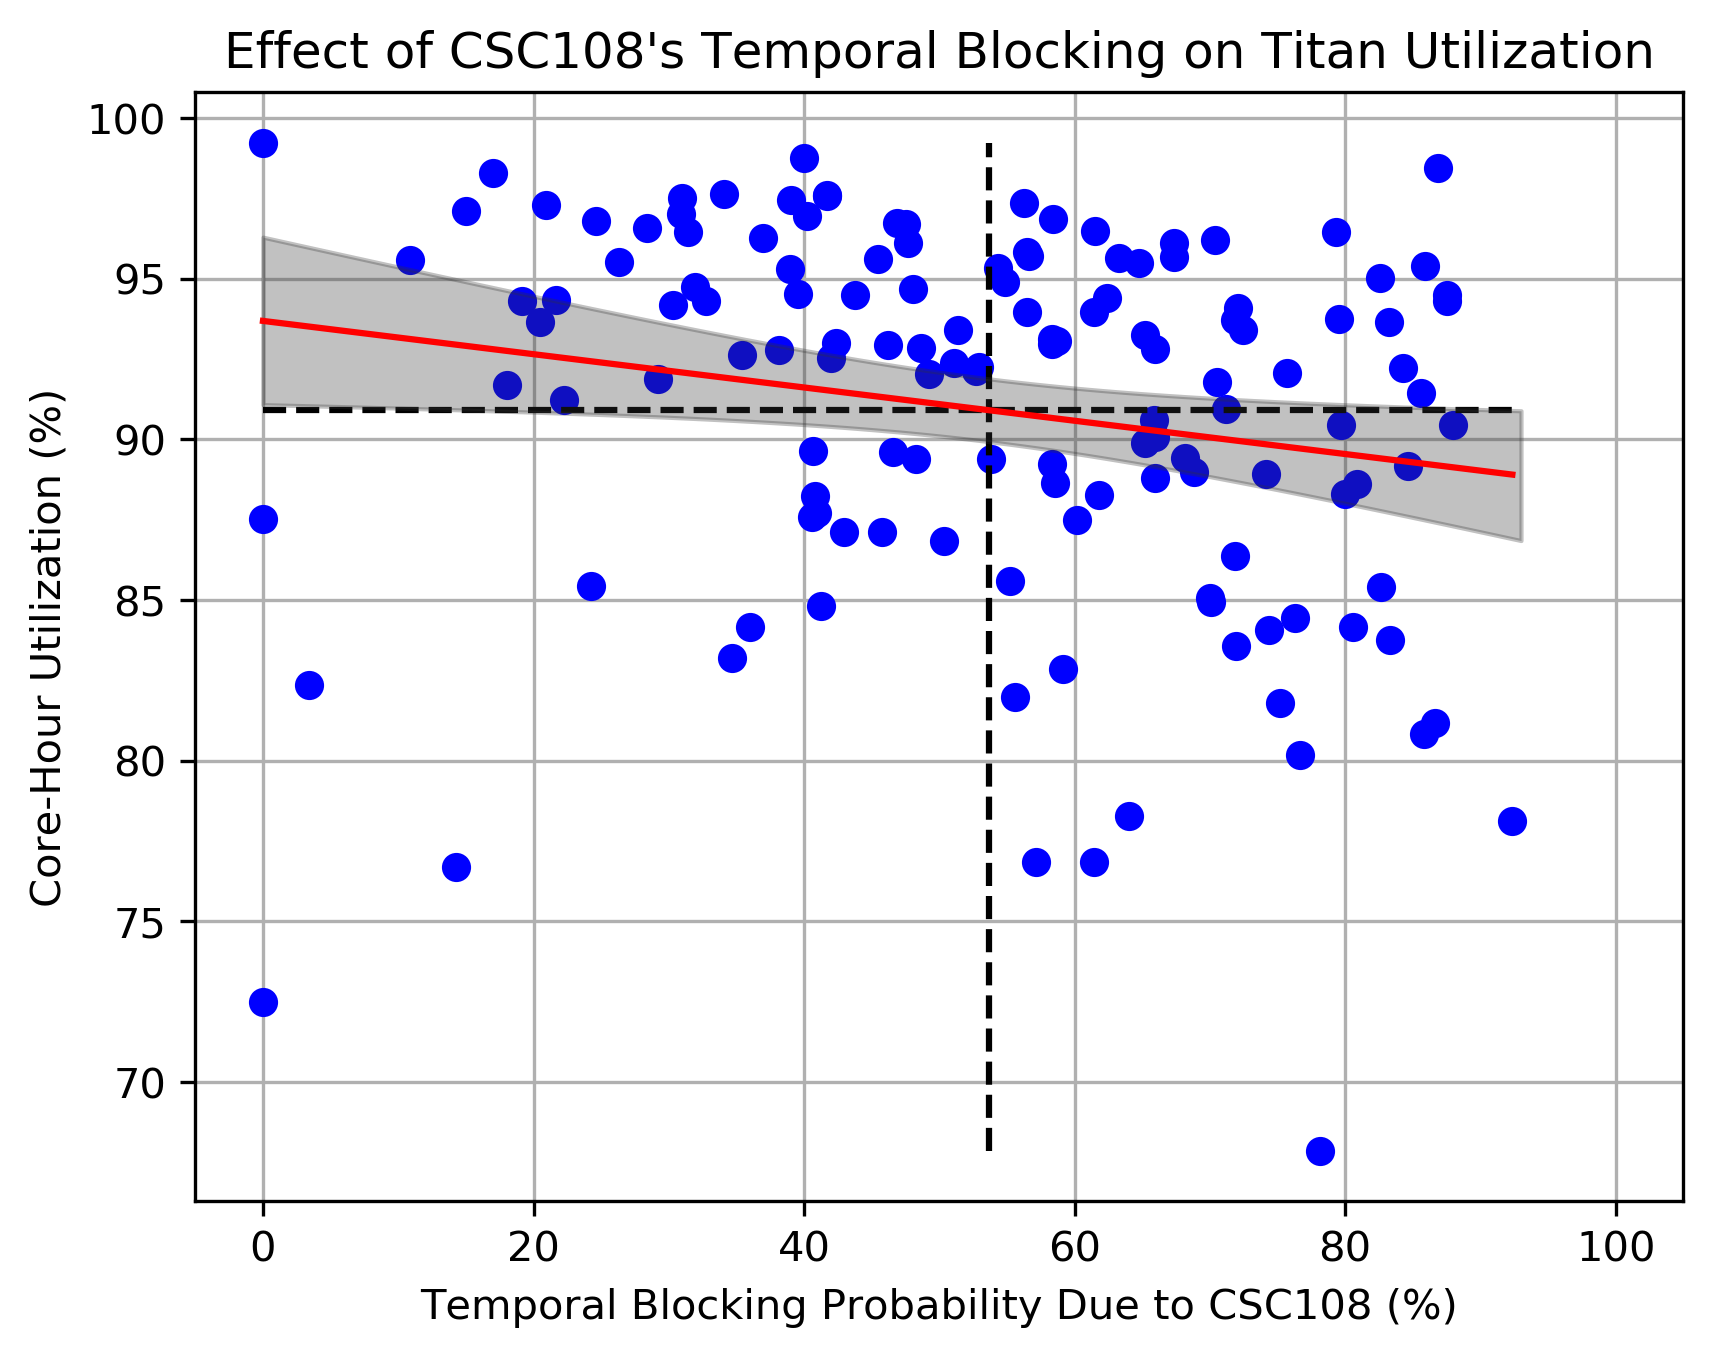
\includegraphics[width=0.4\textwidth]{images/linfit-utilization-vs-csc108-temporal.png}}
  \caption{These plots demonstrate the relationships between utilization on
Titan and one-dimensional blocking probabilities. Each blue point represents
one day. Each red line is an Ordinary Least Squares (OLS) linear regression
with parameters given in Table~\ref{tab:blocking-utilization-params}. Each
shaded gray area represents a 95\% confidence region. Each horizontal dotted
black line represents the mean wait times for all points in that plot, and each
vertical dotted black line represents the mean blocking probability for all
points in that plot.}
\end{figure*}

% For tables use
\begin{table}
% table caption is above the table
\caption{The table contains the parameter values for the Ordinary Least Squares
(OLS) linear regression models regarding blocking probabilities and utilization.
The first column corresponds to the figure depicting the model, while the
second and third columns correspond the coefficients $\beta_1$ and $\beta_0$ in
the model $y = \beta_{1}x + \beta_0$.}
\label{tab:blocking-utilization-params}       % Give a unique label
% For LaTeX tables use
\begin{tabular}{crrr}
\hline\noalign{\smallskip}
Figure  & Slope $\beta_1$ & Intercept $\beta_0$     & $\text{R}^2$ \\
\noalign{\smallskip}\hline\noalign{\smallskip}
\ref{fig:utilization-spatial-all}       &   -0.3766 &   123.8332 & 0.1543 \\
\ref{fig:utilization-temporal-all}    &     -0.1654 &   103.1603 & 0.2084 \\
\ref{fig:utilization-spatial-csc108}  &      0.0617 &    86.5830 & 0.0391 \\
\ref{fig:utilization-temporal-csc108} &     -0.0518 &    93.6845 & 0.0370 \\
\noalign{\smallskip}\hline
\end{tabular}
\end{table}
%%%

Thus, the use of blocking probability provided additional insight regarding the
impact of CSC108 on Titan, but just like in
Section~\ref{subsec:simple-linear-relationships}, the best-fit lines all
displayed very poor goodness-of-fit, rendering the interpretations somewhat
weak.

%-  vim:set syntax=tex:
